% ============================================================================
% CAPÍTULO 4: A MATEMÁTICA DOS SISTEMAS BIOLÓGICOS
% Bioinformática para Biologia de Sistemas
% ============================================================================

% ============================================================================
% TEMPLATE BASE PARA APRESENTAÇÕES EM BEAMER
% Bioinformática para Biologia de Sistemas
% ============================================================================

\documentclass[12pt, aspectratio=169]{beamer}

% ============================================================================
% PACOTES ESSENCIAIS
% ============================================================================
\usepackage[utf8]{inputenc}
\usepackage[T1]{fontenc}
\usepackage[brazilian]{babel}
\usepackage{amsmath, amssymb, amsthm}
\usepackage{graphicx}
\usepackage{xcolor}
\usepackage{tikz}
\usetikzlibrary{arrows.meta, shapes, positioning, calc, decorations.pathreplacing, decorations.shapes, decorations.pathmorphing}
\usepackage{listings}
\usepackage{booktabs}
\usepackage{multirow}
\usepackage{hyperref}
\usepackage{chemfig}
\usepackage{chemarr}

% ============================================================================
% CONFIGURAÇÃO DO TEMA
% ============================================================================
\usetheme{Madrid}
\usecolortheme{default}

% Cores personalizadas
\definecolor{azulescuro}{RGB}{0, 51, 102}
\definecolor{azulclaro}{RGB}{51, 153, 255}
\definecolor{verdeacido}{RGB}{102, 204, 0}
\definecolor{laranjacel}{RGB}{255, 153, 51}
\definecolor{roxodna}{RGB}{153, 51, 255}

\setbeamercolor{structure}{fg=azulescuro}
\setbeamercolor{palette primary}{bg=azulescuro,fg=white}
\setbeamercolor{palette secondary}{bg=azulclaro,fg=white}
\setbeamercolor{palette tertiary}{bg=azulescuro,fg=white}
\setbeamercolor{palette quaternary}{bg=azulclaro,fg=white}
\setbeamercolor{block title}{bg=azulescuro,fg=white}
\setbeamercolor{block body}{bg=azulclaro!10,fg=black}
\setbeamercolor{block title alerted}{bg=red!80,fg=white}
\setbeamercolor{block body alerted}{bg=red!10,fg=black}
\setbeamercolor{block title example}{bg=verdeacido!80,fg=white}
\setbeamercolor{block body example}{bg=verdeacido!10,fg=black}

% ============================================================================
% CONFIGURAÇÃO DE CÓDIGO
% ============================================================================
\lstset{
    language=Python,
    basicstyle=\ttfamily\small,
    keywordstyle=\color{azulescuro}\bfseries,
    commentstyle=\color{verdeacido},
    stringstyle=\color{laranjacel},
    numbers=left,
    numberstyle=\tiny\color{gray},
    stepnumber=1,
    numbersep=5pt,
    backgroundcolor=\color{white},
    showspaces=false,
    showstringspaces=false,
    showtabs=false,
    frame=single,
    rulecolor=\color{black},
    tabsize=2,
    captionpos=b,
    breaklines=true,
    breakatwhitespace=false,
    escapeinside={\%*}{*)},
    xleftmargin=10pt,
    xrightmargin=10pt
}

% Definir estilo para R
\lstdefinestyle{Rstyle}{
    language=R,
    basicstyle=\ttfamily\small,
    keywordstyle=\color{azulescuro}\bfseries,
    commentstyle=\color{verdeacido},
    stringstyle=\color{laranjacel}
}

% Definir estilo para MATLAB
\lstdefinestyle{MATLABstyle}{
    language=Matlab,
    basicstyle=\ttfamily\small,
    keywordstyle=\color{azulescuro}\bfseries,
    commentstyle=\color{verdeacido},
    stringstyle=\color{laranjacel}
}

% ============================================================================
% COMANDOS PERSONALIZADOS
% ============================================================================

% Comando para equações destacadas
\newcommand{\destaque}[1]{%
    \begin{alertblock}{}
        \begin{center}
            #1
        \end{center}
    \end{alertblock}
}

% Comando para definições
\newcommand{\definicao}[2]{%
    \begin{block}{Definição: #1}
        #2
    \end{block}
}

% Comando para exemplos
\newcommand{\exemplo}[2]{%
    \begin{exampleblock}{Exemplo: #1}
        #2
    \end{exampleblock}
}

% Comando para observações importantes
\newcommand{\importante}[1]{%
    \begin{alertblock}{Importante!}
        #1
    \end{alertblock}
}

% Comandos matemáticos úteis
\newcommand{\R}{\mathbb{R}}
\newcommand{\N}{\mathbb{N}}
\newcommand{\Z}{\mathbb{Z}}
\newcommand{\dif}{\mathrm{d}}
\newcommand{\parcial}[2]{\frac{\partial #1}{\partial #2}}
\newcommand{\derivada}[2]{\frac{\dif #1}{\dif #2}}
\newcommand{\vect}[1]{\boldsymbol{#1}}

% Comandos biológicos
\newcommand{\gene}[1]{\textit{#1}}
\newcommand{\proteina}[1]{\textsc{#1}}
\newcommand{\especie}[1]{\textit{#1}}

% ============================================================================
% CONFIGURAÇÃO DE RODAPÉ
% ============================================================================
\setbeamertemplate{footline}{
  \leavevmode%
  \hbox{%
  \begin{beamercolorbox}[wd=.33\paperwidth,ht=2.25ex,dp=1ex,center]{author in head/foot}%
    \usebeamerfont{author in head/foot}\insertshortauthor
  \end{beamercolorbox}%
  \begin{beamercolorbox}[wd=.34\paperwidth,ht=2.25ex,dp=1ex,center]{title in head/foot}%
    \usebeamerfont{title in head/foot}\insertshorttitle
  \end{beamercolorbox}%
  \begin{beamercolorbox}[wd=.33\paperwidth,ht=2.25ex,dp=1ex,right]{date in head/foot}%
    \usebeamerfont{date in head/foot}\insertshortdate{}\hspace*{2em}
    \insertframenumber{} / \inserttotalframenumber\hspace*{2ex}
  \end{beamercolorbox}}%
  \vskip0pt%
}

% ============================================================================
% CONFIGURAÇÃO DE NAVEGAÇÃO
% ============================================================================
\setbeamertemplate{navigation symbols}{}

% ============================================================================
% CONFIGURAÇÃO DE ITEMIZE/ENUMERATE
% ============================================================================
\setbeamertemplate{itemize items}[circle]
\setbeamertemplate{enumerate items}[default]

% ============================================================================
% FIM DO TEMPLATE
% ============================================================================


% ============================================================================
% INFORMAÇÕES DO DOCUMENTO
% ============================================================================
\title[Cap. 4: Matemática de Sistemas Biológicos]{Capítulo 4: A Matemática dos Sistemas Biológicos}
\subtitle{Bioinformática para Biologia de Sistemas}
\author{Ney Lemke}
\institute{DBF-Unesp}
\date{\today}

\begin{document}

% ============================================================================
% SLIDE DE TÍTULO
% ============================================================================
\begin{frame}[allowframebreaks]
\titlepage
\end{frame}

% ============================================================================
% SUMÁRIO
% ============================================================================
\begin{frame}[allowframebreaks]{Sumário}
\tableofcontents
\end{frame}

% ============================================================================
% SEÇÃO 1: INTRODUÇÃO
% ============================================================================
\section{Introdução}

\begin{frame}[allowframebreaks]{Visão Geral do Capítulo}
\begin{block}{Objetivos de Aprendizagem}
\begin{itemize}
    \item Dominar ferramentas matemáticas avançadas para sistemas biológicos
    \item Compreender sistemas de equações diferenciais ordinárias (EDOs)
    \item Realizar análise de estabilidade e linearização
    \item Estudar bifurcações e transições de comportamento
    \item Analisar oscilações e ciclos limite
    \item Aplicar análise de sensibilidade paramétrica
\end{itemize}
\end{block}

\vspace{0.5cm}

\begin{exampleblock}{Por que Matemática Avançada?}
A matemática é essencial para:
\begin{itemize}
    \item Predizer comportamento dinâmico de sistemas
    \item Identificar transições críticas e pontos de decisão
    \item Compreender robustez e sensibilidade
    \item Projetar intervenções terapêuticas eficazes
\end{itemize}
\end{exampleblock}
\end{frame}

\begin{frame}[allowframebreaks]{Matemática como Linguagem da Biologia}
\definicao{Modelagem Matemática}{
A modelagem matemática traduz processos biológicos em equações que capturam a essência dinâmica do sistema, permitindo simulação, análise e predição quantitativas.
}

\vspace{0.3cm}

\begin{columns}
\column{0.48\textwidth}
\textbf{Níveis de Complexidade:}
\begin{itemize}
    \item Modelos lineares (simples)
    \item Sistemas não-lineares (realistas)
    \item Modelos estocásticos (com ruído)
    \item Modelos espaciais (PDEs)
\end{itemize}

\column{0.48\textwidth}
\textbf{Ferramentas Principais:}
\begin{itemize}
    \item Equações diferenciais
    \item Análise de estabilidade
    \item Teoria de bifurcações
    \item Métodos numéricos
\end{itemize}
\end{columns}

\vspace{0.3cm}

\importante{
Este capítulo foca em sistemas dinâmicos determinísticos descritos por EDOs
}
\end{frame}

\begin{frame}{Visão Integrada: Do Modelo à Predição}
\begin{center}
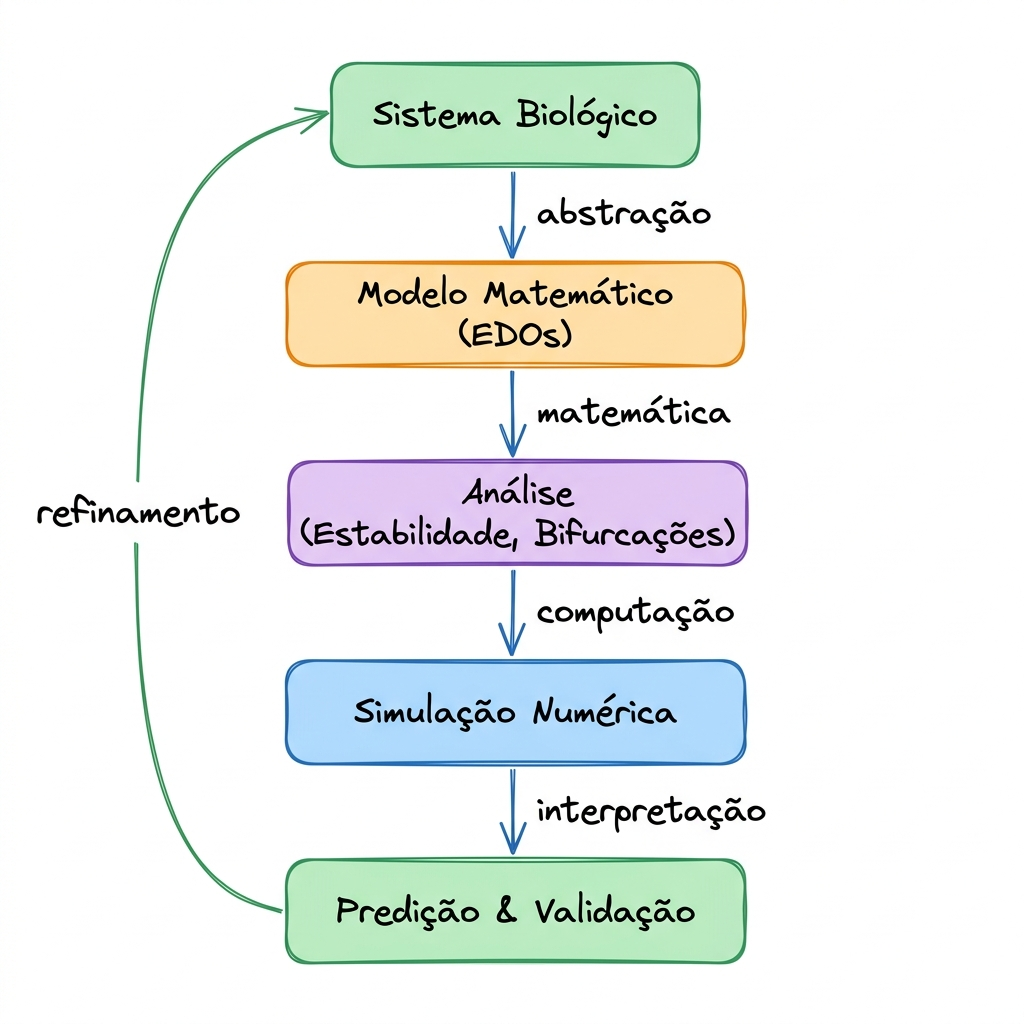
\includegraphics[height=0.72\textheight,keepaspectratio]{images/diagrama_modelagem.png}
\end{center}
\end{frame}

\begin{frame}[allowframebreaks]{Tópicos Avançados deste Capítulo}
\begin{columns}
\column{0.48\textwidth}
\begin{block}{Parte I: Modelagem Discreta}
\begin{enumerate}
    \item Modelos discretos e recursivos
    \item O mapa logístico e estabilidade
    \item Processos estocásticos e ramificação
\end{enumerate}
\end{block}

\begin{block}{Parte II: Dinâmica Contínua}
\begin{enumerate}
    \setcounter{enumi}{3}
    \item Sistemas de EDOs e retratos de fase
    \item Análise de estabilidade e Jacobiano
\end{enumerate}
\end{block}

\column{0.48\textwidth}
\begin{block}{Parte III: Transições e Sensibilidade}
\begin{enumerate}
    \setcounter{enumi}{5}
    \item Bifurcações
    \item Oscilações e ciclos limite
    \item Análise de sensibilidade
\end{enumerate}
\end{block}

\begin{exampleblock}{Aplicações Práticas}
\begin{itemize}
    \item Crescimento populacional e caos
    \item Cadeias de Markov em biologia
    \item Lotka-Volterra e Van der Pol
    \item Sensibilidade local e global
\end{itemize}
\end{exampleblock}
\end{columns}
\end{frame}

% ============================================================================
% SEÇÃO 2: MODELOS DISCRETOS E RECURSIVOS
% ============================================================================
\section{Modelos Discretos e Recursivos}

\begin{frame}[allowframebreaks]{Introdução aos Modelos Discretos}
\definicao{Sistema Dinâmico em Tempo Discreto}{
Um modelo onde o tempo progride em passos inteiros discretos ($t = 0, 1, 2, \ldots$). É descrito por uma relação de recorrência ou equação de diferenças:
\begin{equation*}
x_{t+1} = f(x_t)
\end{equation*}
onde $f$ mapeia o estado atual no próximo estado.
}

\begin{block}{Relevância Biológica}
Muitos processos ocorrem naturalmente em etapas discretas:
\begin{itemize}
    \item \textbf{Gerações não-sobrepostas}: Ciclos de vida anuais de insetos ou plantas sazonais.
    \item \textbf{Divisão Celular Sincronizada}: Populações de células duplicando em intervalos fixos.
    \item \textbf{Replicação Viral}: Ciclos discretos de infecção celular e liberação de vírions.
    \item \textbf{Dados Experimentais}: Medições em pontos fixos (ex: coletas diárias de dados populacionais).
\end{itemize}
\end{block}
\end{frame}

\begin{frame}[allowframebreaks]{Modelos Recursivos Determinísticos: O Mapa Logístico}
\begin{block}{Crescimento Populacional Discreto}
Proposto por Robert May (1976), o \textbf{Mapa Logístico} descreve a dinâmica de uma população sob restrição de recursos em tempo discreto:
\begin{equation*}
x_{t+1} = r x_t (1 - x_t)
\end{equation*}
onde $x_t \in [0, 1]$ representa a densidade populacional e $r > 0$ é a taxa de crescimento.
\end{block}

\begin{exampleblock}{Comportamentos Emergentes com a Variação de $r$}
\begin{itemize}
    \item $0 < r < 1$: Extinção da população ($x_t \to 0$).
    \item $1 < r < 3$: Estabilização em um ponto fixo estável $x^* = 1 - 1/r$.
    \item $3 < r < 3.44$: Ciclo estável de período 2 (oscilação entre dois valores).
    \item $3.44 < r < 3.57$: Duplicação de período (surgimento de ciclos de período 4, 8, 16...).
    \item $r > 3.57$: \textbf{Caos Determinístico} (trajetórias aperiódicas e extrema sensibilidade às condições iniciais).
\end{itemize}
\end{exampleblock}
\end{frame}

\begin{frame}[allowframebreaks]{Estabilidade de Pontos Fixos Discretos}
\definicao{Ponto Fixo Discreto}{
Um ponto $x^*$ é um equilíbrio de $x_{t+1} = f(x_t)$ se $f(x^*) = x^*$.
}

\begin{block}{Critério de Estabilidade Linear}
O equilíbrio discreto $x^*$ é estável se uma pequena perturbação $\xi_t = x_t - x^*$ diminuir em magnitude ao longo do tempo. Expandindo por série de Taylor:
\begin{equation*}
\xi_{t+1} \approx f'(x^*) \xi_t \quad \Rightarrow \quad \xi_t \approx [f'(x^*)]^t \xi_0
\end{equation*}
\end{block}

\importante{
\textbf{Critério de Estabilidade}:
\begin{itemize}
    \item Se $|f'(x^*)| < 1$ $\Rightarrow$ \textbf{estável} (convergência para o ponto fixo).
    \item Se $|f'(x^*)| > 1$ $\Rightarrow$ \textbf{instável} (divergência ou oscilação crescente).
\end{itemize}
}
\end{frame}

\begin{frame}[allowframebreaks]{Modelos Recursivos Estocásticos: Ruído}
\definicao{Estocasticidade}{
Sistemas biológicos operam sob ruído e flutuações, que podem ser incorporados adicionando variáveis aleatórias ao modelo recursivo.
}

\begin{columns}
\column{0.48\textwidth}
\begin{block}{Ruído Aditivo}
Mente perturbações externas constantes (ruído ambiental):
\begin{equation*}
x_{t+1} = f(x_t) + \eta_t
\end{equation*}
onde $\eta_t \sim \mathcal{N}(0, \sigma^2)$ é ruído branco gaussiano.
\end{block}

\column{0.48\textwidth}
\begin{block}{Ruído Multiplicativo}
Mente flutuações proporcionais à própria população (estocasticidade demográfica):
\begin{equation*}
x_{t+1} = f(x_t) \cdot e^{\eta_t}
\end{equation*}
\end{block}
\end{columns}

\vspace{0.2cm}
\importante{
O ruído estocástico impede que o sistema permaneça exatamente em um ponto fixo, gerando uma distribuição estatística de estados em torno dele.
}
\end{frame}

\begin{frame}{Cadeias de Markov de Tempo Discreto}
\definicao{Cadeia de Markov Discreta (DTMC)}{
Processo estocástico sem memória, onde a probabilidade de transição depende apenas do estado atual:
\begin{equation*}
P(X_{t+1} = j \mid X_t = i, X_{t-1} = i_{t-1}, \ldots) = P_{ij}
\end{equation*}
}

\begin{block}{Evolução Probabilística Recursiva}
Dada a matriz de transição $\vect{P}$ (onde $\sum_{j} P_{ij} = 1$) e o vetor de estados $\vect{p}(t)$:
\begin{equation*}
\vect{p}(t+1) = \vect{P} \cdot \vect{p}(t) \quad \Rightarrow \quad \vect{p}(t) = \vect{P}^t \vect{p}(0)
\end{equation*}
\end{block}
\end{frame}

\begin{frame}{Cadeias de Markov: Distribuição Estacionária}
\definicao{Distribuição Estacionária ($\vect{\pi}$)}{
É o vetor de probabilidades $\vect{\pi}$ que permanece invariante após um passo de transição da cadeia de Markov:
\begin{equation*}
\vect{\pi} = \vect{P}^T \vect{\pi} \quad \text{ou} \quad \pi_j = \sum_{i} \pi_i P_{ij}
\end{equation*}
sujeito à normalização: $\sum_{i} \pi_i = 1$.
}

\vspace{0.2cm}

\begin{exampleblock}{Comportamento Assintótico (Longo Prazo)}
Para cadeias irredutíveis e aperiódicas (ergódicas), o sistema converge para a distribuição estacionária independente do estado inicial:
\begin{equation*}
\lim_{t \to \infty} \vect{p}(t) = \vect{\pi}
\end{equation*}
\end{exampleblock}
\end{frame}

\begin{frame}{Cadeias de Markov: Exemplo de Canal Iônico}
\begin{columns}
\column{0.48\textwidth}
\textbf{Matriz de Transição $\vect{P}$:}
\begin{equation*}
\vect{P} = \begin{bmatrix}
1 - \alpha & \alpha \\
\beta & 1 - \beta
\end{bmatrix}
\end{equation*}
onde:
\begin{itemize}
    \item $\alpha$: prob. de abrir ($F \to A$)
    \item $\beta$: prob. de fechar ($A \to F$)
\end{itemize}

\column{0.48\textwidth}
\textbf{Distribuição Estacionária ($\vect{\pi}$):}
Resolve-se $\vect{\pi} \vect{P} = \vect{\pi}$:
\begin{align*}
\pi_F &= \frac{\beta}{\alpha + \beta} \\
\pi_A &= \frac{\alpha}{\alpha + \beta}
\end{align*}
$\pi_A$ é a fração de canais abertos no equilíbrio!
\end{columns}

\vspace{0.1cm}
\begin{center}
\begin{tikzpicture}[auto, scale=0.75, transform shape, >=stealth]
    \node[circle, draw, fill=laranjacel!20, minimum size=1.6cm, align=center, draw=laranjacel!80, thick] (F) {Fechado\\(F)};
    \node[circle, draw, fill=azulclaro!20, minimum size=1.6cm, align=center, right=1.6cm of F, draw=azulclaro!80, thick] (A) {Aberto\\(A)};
    \path[->, thick]
        (F) edge [bend left=25, draw=roxodna] node {$\alpha$} (A)
        (A) edge [bend left=25, draw=roxodna] node {$\beta$} (F)
        (F) edge [loop left, looseness=8, draw=laranjacel] node {$1-\alpha$} (F)
        (A) edge [loop right, looseness=8, draw=azulclaro] node {$1-\beta$} (A);
\end{tikzpicture}
\end{center}
\end{frame}

\begin{frame}[allowframebreaks]{Processos de Ramificação (Galton-Watson)}
\definicao{Processo de Galton-Watson}{
Modelo estocástico clássico para o tamanho de populações que se reproduzem de forma discreta e independente:
\begin{equation*}
Z_{t+1} = \sum_{i=1}^{Z_t} Y_i^{(t)}
\end{equation*}
onde $Z_t$ é a população no tempo $t$, e $Y_i^{(t)}$ é uma variável aleatória que representa o número de descendentes gerados pelo indivíduo $i$.
}

\begin{block}{Propriedades de Sobrevivência e Extinção}
Seja $m = E[Y]$ o número médio de descendentes por indivíduo:
\begin{itemize}
    \item \textbf{Subcrítico} ($m < 1$): A população entra em extinção com probabilidade 1.
    \item \textbf{Crítico} ($m = 1$): A população entra em extinção com probabilidade 1 (a menos que $P(Y=1)=1$).
    \item \textbf{Supercrítico} ($m > 1$): Há uma probabilidade positiva de sobrevivência infinita.
\end{itemize}
\end{block}
\end{frame}

\begin{frame}[fragile, allowframebreaks]{Simulando Sistemas Discretos (Python)}
\begin{lstlisting}[language=Python, basicstyle=\ttfamily\footnotesize]
import numpy as np
import matplotlib.pyplot as plt

# Parametros do Mapa Logistico
r = 3.8       # Comportamento caotico
sigma = 0.02  # Intensidade do ruido estocastico
steps = 50
x_det = np.zeros(steps)
x_est = np.zeros(steps)
x_det[0] = x_est[0] = 0.5

# Simulacao Recursiva
for t in range(steps - 1):
    # Determinista
    x_det[t+1] = r * x_det[t] * (1 - x_det[t])
    # Estocastico com ruido multiplicativo (truncado em 0 e 1)
    noise = np.random.normal(0, sigma)
    val = r * x_est[t] * (1 - x_est[t]) * np.exp(noise)
    x_est[t+1] = np.clip(val, 0.0, 1.0)

# Visualizar
plt.figure(figsize=(10, 4))
plt.plot(x_det, 'b-o', label='Determinista')
plt.plot(x_est, 'r--x', label='Estocastico')
plt.xlabel('Tempo (t)')
plt.ylabel('Populacao x(t)')
plt.legend()
plt.grid(True)
\end{lstlisting}
\end{frame}

% ============================================================================
% SEÇÃO 3: SISTEMAS DE EQUAÇÕES DIFERENCIAIS
% ============================================================================
\section{Sistemas de Equações Diferenciais}

\begin{frame}{Revisão: Equações Diferenciais Ordinárias}
\definicao{Equação Diferencial Ordinária (EDO)}{
Uma EDO relaciona uma função desconhecida $y(t)$ com suas derivadas:
\begin{equation*}
\frac{dy}{dt} = f(y, t)
\end{equation*}
onde $t$ é a variável independente (geralmente tempo) e $y$ é a variável dependente.
}

\vspace{0.6cm}

\importante{
Sistemas biológicos geralmente requerem sistemas de EDOs acopladas!
}
\end{frame}

\begin{frame}{Revisão: Exemplos de EDOs}
\begin{columns}
\column{0.48\textwidth}
\begin{exampleblock}{EDO de 1ª Ordem}
\begin{equation*}
\frac{dx}{dt} = -kx
\end{equation*}
Solução: $x(t) = x_0 e^{-kt}$\\
(decaimento exponencial)
\end{exampleblock}

\column{0.48\textwidth}
\begin{exampleblock}{EDO de 2ª Ordem}
\begin{equation*}
\frac{d^2x}{dt^2} + \omega^2 x = 0
\end{equation*}
Solução: $x(t) = A\cos(\omega t) + B\sin(\omega t)$\\
(oscilador harmônico)
\end{exampleblock}
\end{columns}
\end{frame}

\begin{frame}[allowframebreaks]{Sistemas de EDOs Não-Lineares}
\begin{block}{Forma Geral}
Um sistema de $n$ equações diferenciais de primeira ordem:
\begin{align*}
\frac{dx_1}{dt} &= f_1(x_1, x_2, \ldots, x_n, t)\\
\frac{dx_2}{dt} &= f_2(x_1, x_2, \ldots, x_n, t)\\
&\vdots\\
\frac{dx_n}{dt} &= f_n(x_1, x_2, \ldots, x_n, t)
\end{align*}
\end{block}

\textbf{Forma Vetorial:}
\begin{equation*}
\frac{d\vect{x}}{dt} = \vect{f}(\vect{x}, t)
\end{equation*}
onde $\vect{x} = (x_1, x_2, \ldots, x_n)^T$ e $\vect{f} = (f_1, f_2, \ldots, f_n)^T$

\vspace{0.3cm}

\textbf{Sistema Autônomo:} quando $\vect{f}$ não depende explicitamente de $t$
\end{frame}

\begin{frame}{Campos Vetoriais e Retratos de Fase}
\definicao{Campo Vetorial}{
O lado direito do sistema $\vect{f}(\vect{x})$ define um campo vetorial que associa a cada ponto do espaço de estados um vetor velocidade.
}

\vspace{0.15cm}

\begin{columns}
\column{0.48\textwidth}
\textbf{Exemplo Simples:} \\
$\frac{dx}{dt} = y, \quad \frac{dy}{dt} = -x$

\vspace{0.2cm}

\textbf{Interpretação:}
\begin{itemize}
    \item Em cada ponto $(x,y)$ existe um vetor $(\dot{x}, \dot{y})$
    \item As soluções seguem as linhas de fluxo
    \item O conjunto de todas as trajetórias forma o retrato de fase
\end{itemize}

\column{0.48\textwidth}
\begin{center}
\begin{tikzpicture}[scale=0.7]
    % Eixos
    \draw[->] (-2,0) -- (2,0) node[right] {$x$};
    \draw[->] (0,-2) -- (0,2) node[above] {$y$};

    % Campo vetorial
    \foreach \x in {-1.5,-0.75,0,0.75,1.5}
        \foreach \y in {-1.5,-0.75,0,0.75,1.5}
            \draw[->, azulescuro, thick] (\x,\y) -- ++(0.15*\y, -0.15*\x);

    % Trajetória circular
    \draw[verdeacido, thick, ->] (1,0) arc[start angle=0, end angle=270, radius=1];

    \node[below] at (0,-2.1) {\small Oscilador Harmônico};
\end{tikzpicture}
\end{center}
\end{columns}
\end{frame}

\begin{frame}[allowframebreaks]{Nulclinas}
\definicao{Nulclina}{
Curva no espaço de fase onde uma das derivadas é zero:
\begin{itemize}
    \item \textbf{x-nulclina:} onde $\dot{x} = 0$ (movimento apenas vertical)
    \item \textbf{y-nulclina:} onde $\dot{y} = 0$ (movimento apenas horizontal)
\end{itemize}
}

\vspace{0.3cm}

\begin{center}
\begin{tikzpicture}[scale=0.9]
    % Eixos
    \draw[->] (-0.5,0) -- (4,0) node[right] {$x$};
    \draw[->] (0,-0.5) -- (0,3) node[above] {$y$};

    % x-nulclina (dy/dt = 0)
    \draw[thick, verdeacido, domain=0:3.5] plot (\x, {2 - 0.5*\x}) node[right] {$\dot{y}=0$};

    % y-nulclina (dx/dt = 0)
    \draw[thick, roxodna, domain=0:2.5] plot (\x, {0.6*\x}) node[above right] {$\dot{x}=0$};

    % Ponto de equilibrio
    \fill[red] (1.6, 0.96) circle (2pt) node[above right] {$(x^*, y^*)$};

    % Setas de direcao
    \draw[->, thick] (0.5, 2.5) -- (1, 2.5);
    \draw[->, thick] (3, 0.5) -- (3, 1);

    \node[below] at (2,-1) {Nulclinas se cruzam no equilíbrio};
\end{tikzpicture}
\end{center}

\importante{
Pontos de equilíbrio ocorrem na interseção das nulclinas!
}
\end{frame}

\begin{frame}[allowframebreaks]{Campos de Direção}
\begin{block}{Construindo Retratos de Fase}
\begin{enumerate}
    \item Calcular e plotar nulclinas ($\dot{x}=0$ e $\dot{y}=0$)
    \item Identificar pontos de equilíbrio (interseções)
    \item Desenhar campo de direções (vetores $(\dot{x}, \dot{y})$)
    \item Integrar trajetórias numéricas a partir de condições iniciais
    \item Analisar comportamento assintótico
\end{enumerate}
\end{block}

\vspace{0.3cm}

\begin{center}
\begin{tikzpicture}[scale=0.7]
    % Eixos
    \draw[->] (-3,0) -- (3,0) node[right] {$x$};
    \draw[->] (0,-2) -- (0,2) node[above] {$y$};

    % Campo de direcoes
    \foreach \x in {-2.5,-1.5,-0.5,0.5,1.5,2.5}
        \foreach \y in {-1.5,-0.5,0.5,1.5} {
            \pgfmathsetmacro{\dx}{\y}
            \pgfmathsetmacro{\dy}{-\x - 0.3*\y}
            \pgfmathsetmacro{\norm}{sqrt(\dx*\dx + \dy*\dy)}
            \pgfmathsetmacro{\scale}{0.15}
            \draw[->, gray] (\x,\y) -- ++(\scale*\dx/\norm, \scale*\dy/\norm);
        }

    % Trajetoria exemplo
    \draw[thick, azulescuro, ->] (2,1.5) .. controls (1,1) and (0.5,0) .. (0,-0.5);
    \draw[thick, verdeacido, ->] (-2,-1) .. controls (-1,0) and (-0.5,0.5) .. (0,0.5);

    % Equilibrio
    \fill[red] (0,0) circle (2pt);
\end{tikzpicture}
\end{center}
\end{frame}

\begin{frame}[fragile,allowframebreaks]{Resolvendo EDOs com SciPy}
\begin{lstlisting}[language=Python, caption=Sistema de EDOs com scipy.integrate, basicstyle=\ttfamily\footnotesize]
import numpy as np
from scipy.integrate import odeint
import matplotlib.pyplot as plt

# Definir sistema de EDOs
def sistema(X, t, alpha, beta):
    """Sistema de duas variaveis acopladas"""
    x, y = X
    dxdt = alpha*x - beta*x*y
    dydt = -y + x*y
    return [dxdt, dydt]

# Parametros
alpha = 1.0
beta = 0.5

# Condicao inicial
X0 = [2.0, 1.0]

# Tempo
t = np.linspace(0, 20, 1000)

# Resolver
sol = odeint(sistema, X0, t, args=(alpha, beta))

# Plotar series temporal
plt.figure(figsize=(10, 4))
plt.plot(t, sol[:, 0], 'b-', label='x(t)')
plt.plot(t, sol[:, 1], 'r-', label='y(t)')
plt.xlabel('Tempo')
plt.ylabel('Concentracao')
plt.legend()
plt.grid(True)
\end{lstlisting}
\end{frame}

\begin{frame}[allowframebreaks]{Exemplo: Modelo Lotka-Volterra}
\begin{block}{Sistema Predador-Presa}
\begin{align*}
\frac{dx}{dt} &= \alpha x - \beta xy \quad \text{(presas)}\\
\frac{dy}{dt} &= \delta xy - \gamma y \quad \text{(predadores)}
\end{align*}
Parâmetros:
\begin{itemize}
    \item $\alpha$: taxa de crescimento das presas
    \item $\beta$: taxa de predação
    \item $\delta$: eficiência de conversão
    \item $\gamma$: taxa de morte dos predadores
\end{itemize}
\end{block}

\vspace{0.3cm}

\textbf{Ponto de Equilíbrio:}
\begin{equation*}
x^* = \frac{\gamma}{\delta}, \quad y^* = \frac{\alpha}{\beta}
\end{equation*}

\importante{
Este sistema exibe oscilações periódicas (órbitas fechadas)!
}
\end{frame}

\begin{frame}[allowframebreaks]{Retrato de Fase do Lotka-Volterra}
\begin{columns}
\column{0.48\textwidth}
\textbf{Características:}
\begin{itemize}
    \item Órbitas fechadas (periódicas)
    \item Centro estável em $(x^*, y^*)$
    \item Amplitude depende da condição inicial
    \item Não há atrator: órbitas neutras
    \item Sistema conservativo
\end{itemize}

\vspace{0.3cm}

\textbf{Nulclinas:}
\begin{itemize}
    \item $\dot{x} = 0$: $y = \alpha/\beta$
    \item $\dot{y} = 0$: $x = \gamma/\delta$
\end{itemize}

\column{0.48\textwidth}
\begin{center}
\begin{tikzpicture}[scale=0.8]
    % Eixos
    \draw[->] (0,0) -- (4,0) node[right] {$x$ (presas)};
    \draw[->] (0,0) -- (0,3.5) node[above] {$y$ (pred.)};

    % Nulclinas
    \draw[thick, verdeacido, dashed] (0,2) -- (4,2) node[right, font=\tiny] {$\dot{x}=0$};
    \draw[thick, roxodna, dashed] (2,0) -- (2,3.5) node[above, font=\tiny] {$\dot{y}=0$};

    % Equilibrio
    \fill[red] (2,2) circle (2pt) node[below right, font=\small] {$(x^*, y^*)$};

    % Orbitas fechadas
    \draw[thick, azulescuro] (2,2) ellipse (0.5 and 0.4);
    \draw[thick, azulclaro] (2,2) ellipse (1 and 0.8);
    \draw[thick, azulescuro] (2,2) ellipse (1.5 and 1.2);

    % Setas indicando direcao
    \draw[->, thick] (2.5,2) arc[start angle=0, end angle=45, x radius=0.5, y radius=0.4];
    \draw[->, thick] (3,2) arc[start angle=0, end angle=45, x radius=1, y radius=0.8];
\end{tikzpicture}
\end{center}
\textbf{Interpretação:}\\
Populações oscilam ciclicamente com defasagem temporal
\end{columns}
\end{frame}

\begin{frame}[fragile,allowframebreaks]{Simulando Lotka-Volterra}
\begin{lstlisting}[language=Python, basicstyle=\ttfamily\footnotesize]
import numpy as np
from scipy.integrate import odeint
import matplotlib.pyplot as plt

def lotka_volterra(X, t, alpha, beta, delta, gamma):
    """Modelo predador-presa"""
    x, y = X
    dxdt = alpha*x - beta*x*y
    dydt = delta*x*y - gamma*y
    return [dxdt, dydt]

# Parametros
alpha, beta, delta, gamma = 1.0, 0.5, 0.5, 1.0

# Condicoes iniciais
X0 = [2.0, 1.0]

# Tempo
t = np.linspace(0, 50, 1000)

# Resolver
sol = odeint(lotka_volterra, X0, t, args=(alpha, beta, delta, gamma))

# Plotar retrato de fase
plt.figure(figsize=(8, 6))
plt.plot(sol[:, 0], sol[:, 1], 'b-', linewidth=2)
plt.plot(gamma/delta, alpha/beta, 'ro', markersize=10, label='Equilibrio')
plt.xlabel('Presas (x)')
plt.ylabel('Predadores (y)')
plt.legend()
plt.grid(True)
\end{lstlisting}
\end{frame}

% ============================================================================
% SEÇÃO 4: ANÁLISE DE ESTABILIDADE
% ============================================================================
\section{Análise de Estabilidade}

\begin{frame}[allowframebreaks]{Pontos de Equilíbrio}
\definicao{Ponto de Equilíbrio (Ponto Fixo)}{
Um ponto $\vect{x}^*$ é um ponto de equilíbrio se:
\begin{equation*}
\vect{f}(\vect{x}^*) = \vect{0}
\end{equation*}
Ou seja, todas as derivadas são zero: $\dot{x}_i = 0$ para todo $i$.
}

\vspace{0.3cm}

\begin{exampleblock}{Interpretação Biológica}
Pontos de equilíbrio representam:
\begin{itemize}
    \item Estados estacionários do sistema
    \item Concentrações constantes ao longo do tempo
    \item Homeostase em sistemas biológicos
    \item Possíveis estados finais de longo prazo
\end{itemize}
\end{exampleblock}

\vspace{0.3cm}

\textbf{Questão Central:} O equilíbrio é estável ou instável?
\begin{itemize}
    \item \textbf{Estável:} sistema retorna após pequenas perturbações
    \item \textbf{Instável:} sistema diverge após perturbações
\end{itemize}
\end{frame}

\begin{frame}[allowframebreaks]{Análise de Estabilidade Linear}
\begin{block}{Linearização em torno do Equilíbrio}
Considere pequena perturbação $\vect{\xi}(t) = \vect{x}(t) - \vect{x}^*$:
\begin{equation*}
\frac{d\vect{\xi}}{dt} = \vect{J}(\vect{x}^*) \vect{\xi}
\end{equation*}
onde $\vect{J}$ é a matriz Jacobiana avaliada no equilíbrio.
\end{block}

\vspace{0.3cm}

\definicao{Matriz Jacobiana}{
Matriz das derivadas parciais:
\begin{equation*}
J_{ij} = \frac{\partial f_i}{\partial x_j}\bigg|_{\vect{x}^*}
\end{equation*}

Para sistema 2D:
\begin{equation*}
\vect{J} = \begin{bmatrix}
\frac{\partial f_1}{\partial x_1} & \frac{\partial f_1}{\partial x_2}\\
\frac{\partial f_2}{\partial x_1} & \frac{\partial f_2}{\partial x_2}
\end{bmatrix}_{\vect{x}^*}
\end{equation*}
}
\end{frame}

\begin{frame}[allowframebreaks]{Autovalores e Estabilidade}
\importante{
A estabilidade do equilíbrio $\vect{x}^*$ é determinada pelos autovalores $\lambda_i$ da matriz Jacobiana $\vect{J}(\vect{x}^*)$.
}

\vspace{0.3cm}

\begin{block}{Critério de Estabilidade}
Para cada autovalor $\lambda = a + bi$:
\begin{itemize}
    \item Se $\text{Re}(\lambda_i) < 0$ para todos $i$ $\Rightarrow$ \textbf{estável}
    \item Se $\text{Re}(\lambda_i) > 0$ para algum $i$ $\Rightarrow$ \textbf{instável}
    \item Se $\text{Re}(\lambda_i) = 0$ para algum $i$ $\Rightarrow$ \textbf{marginal} (análise não-linear necessária)
\end{itemize}
\end{block}

\vspace{0.3cm}

\textbf{Equação Característica (2D):}
\begin{equation*}
\det(\vect{J} - \lambda \vect{I}) = 0 \quad \Rightarrow \quad \lambda^2 - \text{tr}(\vect{J})\lambda + \det(\vect{J}) = 0
\end{equation*}
onde $\text{tr}(\vect{J}) = J_{11} + J_{22}$ e $\det(\vect{J}) = J_{11}J_{22} - J_{12}J_{21}$
\end{frame}

\begin{frame}{Classificação de Pontos Fixos em 2D}
\begin{center}
\begin{tikzpicture}[scale=0.9]
    % 1. Preenchimento das Regiões (Fills)
    % Espirais (acima da parábola)
    \fill[azulclaro!15] (-4,4) -- plot[domain=-4:4] (\x, {\x*\x/4}) -- (4,4) -- cycle;
    
    % Nós Estáveis (esquerda)
    \fill[verdeacido!15] (-4,0) -- (-4,4) -- plot[domain=-4:0] (\x, {\x*\x/4}) -- (0,0) -- cycle;
    
    % Nós Instáveis (direita)
    \fill[verdeacido!15] (0,0) -- plot[domain=0:4] (\x, {\x*\x/4}) -- (4,4) -- (4,0) -- cycle;
    
    % Selas (abaixo do eixo tr)
    \fill[laranjacel!10] (-4,-1.0) -- (-4,0) -- (4,0) -- (4,-1.0) -- cycle;

    % 2. Linhas de Divisão e Parábola
    % Parábola: tr^2 = 4*det
    \draw[thick, dashed, draw=black!60] plot[domain=-4:4] (\x, {\x*\x/4});

    % Eixos coordenados
    \draw[->, thick] (-4.5,0) -- (4.5,0) node[right] {$\text{tr}(\vect{J})$};
    \draw[->, thick] (0,-1.2) -- (0,4.2) node[above] {$\det(\vect{J})$};

    % Rótulos da curva da parábola
    \node[rotate=-45, fill=white, inner sep=1pt, font=\tiny, text=black!70] at (-2.8, 1.96) {$\text{tr}^2 = 4\det$};
    \node[rotate=45, fill=white, inner sep=1pt, font=\tiny, text=black!70] at (2.8, 1.96) {$\text{tr}^2 = 4\det$};

    % 3. Rótulos das Regiões
    \node[align=center, font=\small\bfseries, color=azulescuro] at (-1.8, 2.3) {Espirais\\Estáveis};
    \node[align=center, font=\small\bfseries, color=azulescuro] at (1.8, 2.3) {Espirais\\Instáveis};
    
    \node[align=center, font=\small\bfseries, color=verdeacido!50!black] at (-3.1, 0.8) {Nós\\Estáveis};
    \node[align=center, font=\small\bfseries, color=verdeacido!50!black] at (3.1, 0.8) {Nós\\Instáveis};
    
    \node[align=center, font=\small\bfseries, color=laranjacel!80!black] at (-2, -0.5) {Selas};
    \node[align=center, font=\small\bfseries, color=laranjacel!80!black] at (2, -0.5) {Selas};

    % 4. Indicações de Estabilidade Geral
    \node[font=\tiny\bfseries, color=verdeacido!50!black] at (-2.5, 3.7) {ESTÁVEL ($\text{tr} < 0$)};
    \node[font=\tiny\bfseries, color=red!70!black] at (2.5, 3.7) {INSTÁVEL ($\text{tr} > 0$)};
    
    % Rótulos de inequações
    \node[fill=azulclaro!15, inner sep=1pt, font=\tiny, text=black!70] at (0, 3.4) {$\text{tr}^2 < 4\det$};
    \node[fill=verdeacido!15, inner sep=1pt, font=\tiny, text=black!70] at (-2.5, 1.3) {$\text{tr}^2 > 4\det$};
    \node[fill=verdeacido!15, inner sep=1pt, font=\tiny, text=black!70] at (2.5, 1.3) {$\text{tr}^2 > 4\det$};
\end{tikzpicture}
\end{center}
\end{frame}

\begin{frame}{Tipos de Pontos Fixos: Nós}
\begin{columns}
\column{0.48\textwidth}
\begin{block}{1. Nó Estável}
\begin{itemize}
    \item Ambos $\lambda_i < 0$ (reais)
    \item Convergência exponencial
    \item Sem oscilações
\end{itemize}
\begin{center}
\begin{tikzpicture}[scale=0.55]
    \draw[->] (-2,0) -- (2,0);
    \draw[->] (0,-2) -- (0,2);
    \fill[red] (0,0) circle (2pt);
    \foreach \angle in {0,45,90,135,180,225,270,315} {
        \draw[->, thick, azulescuro] ({1.5*cos(\angle)},{1.5*sin(\angle)}) -- ({0.3*cos(\angle)},{0.3*sin(\angle)});
    }
\end{tikzpicture}
\end{center}
\end{block}

\column{0.48\textwidth}
\begin{block}{2. Nó Instável}
\begin{itemize}
    \item Ambos $\lambda_i > 0$ (reais)
    \item Divergência exponencial
    \item Sem oscilações
\end{itemize}
\begin{center}
\begin{tikzpicture}[scale=0.55]
    \draw[->] (-2,0) -- (2,0);
    \draw[->] (0,-2) -- (0,2);
    \fill[red] (0,0) circle (2pt);
    \foreach \angle in {0,45,90,135,180,225,270,315} {
        \draw[->, thick, verdeacido] ({0.3*cos(\angle)},{0.3*sin(\angle)}) -- ({1.5*cos(\angle)},{1.5*sin(\angle)});
    }
\end{tikzpicture}
\end{center}
\end{block}
\end{columns}
\end{frame}

\begin{frame}{Tipos de Pontos Fixos: Sela e Centro}
\begin{columns}
\column{0.48\textwidth}
\begin{block}{3. Ponto de Sela}
\begin{itemize}
    \item $\lambda_1 < 0 < \lambda_2$ (sinais opostos)
    \item Instável (a direção $\lambda_2 > 0$ diverge)
    \item Trajetórias hiperbólicas
\end{itemize}
\begin{center}
\begin{tikzpicture}[scale=0.55]
    \draw[->] (-2,0) -- (2,0);
    \draw[->] (0,-2) -- (0,2);
    \fill[red] (0,0) circle (2pt);
    \draw[->, thick] (1.5,0.3) -- (0.2,0.05);
    \draw[->, thick] (1.5,-0.3) -- (0.2,-0.05);
    \draw[->, thick] (-1.5,0.3) -- (-0.2,0.05);
    \draw[->, thick] (-1.5,-0.3) -- (-0.2,-0.05);
    \draw[->, thick] (0.3,1.5) -- (0.8,1.8);
    \draw[->, thick] (-0.3,1.5) -- (-0.8,1.8);
    \draw[->, thick] (0.3,-1.5) -- (0.8,-1.8);
    \draw[->, thick] (-0.3,-1.5) -- (-0.8,-1.8);
\end{tikzpicture}
\end{center}
\end{block}

\column{0.48\textwidth}
\begin{block}{4. Centro}
\begin{itemize}
    \item $\lambda = \pm i\omega$ (imaginários puros)
    \item Órbitas fechadas oscilatórias
    \item Estável (mas não assintoticamente)
\end{itemize}
\begin{center}
\begin{tikzpicture}[scale=0.55]
    \draw[->] (-2,0) -- (2,0);
    \draw[->] (0,-2) -- (0,2);
    \fill[red] (0,0) circle (2pt);
    \draw[thick, azulclaro] (0,0) circle (0.7);
    \draw[thick, azulclaro] (0,0) circle (1.3);
    \draw[->, thick] (0.7,0) arc[start angle=0, end angle=45, radius=0.7];
\end{tikzpicture}
\end{center}
\end{block}
\end{columns}
\end{frame}

\begin{frame}{Espirais: Estáveis vs. Instáveis}
\begin{columns}
\column{0.48\textwidth}
\begin{block}{Espiral Estável}
\begin{itemize}
    \item $\lambda = a \pm bi$ com $a < 0$
    \item Convergência oscilatória
    \item Período: $T = 2\pi/|b|$
    \item Amortecimento: $e^{at}$
\end{itemize}
\begin{center}
\begin{tikzpicture}[scale=0.4]
    \draw[->] (-1.5,0) -- (1.5,0) node[right] {$x$};
    \draw[->] (0,-1.5) -- (0,1.5) node[above] {$y$};
    \fill[red] (0,0) circle (2pt);
    \draw[thick, azulescuro, domain=0:6*pi, samples=100]
        plot ({exp(-0.1*\x)*cos(\x r)}, {exp(-0.1*\x)*sin(\x r)});
    \draw[->, thick] ({exp(-0.1*2*pi)*cos(2*pi r)}, {exp(-0.1*2*pi)*sin(2*pi r)}) --
                     ({exp(-0.1*2.2*pi)*cos(2.2*pi r)}, {exp(-0.1*2.2*pi)*sin(2.2*pi r)});
\end{tikzpicture}
\end{center}
\end{block}

\column{0.48\textwidth}
\begin{block}{Espiral Instável}
\begin{itemize}
    \item $\lambda = a \pm bi$ com $a > 0$
    \item Divergência oscilatória
    \item Período: $T = 2\pi/|b|$
    \item Crescimento: $e^{at}$
\end{itemize}
\begin{center}
\begin{tikzpicture}[scale=0.4]
    \draw[->] (-1.5,0) -- (1.5,0) node[right] {$x$};
    \draw[->] (0,-1.5) -- (0,1.5) node[above] {$y$};
    \fill[red] (0,0) circle (2pt);
    \draw[thick, verdeacido, domain=0:4*pi, samples=100]
        plot ({exp(0.08*\x)*cos(\x r)}, {exp(0.08*\x)*sin(\x r)});
    \draw[->, thick] ({exp(0.08*2*pi)*cos(2*pi r)}, {exp(0.08*2*pi)*sin(2*pi r)}) --
                     ({exp(0.08*2.2*pi)*cos(2.2*pi r)}, {exp(0.08*2.2*pi)*sin(2.2*pi r)});
\end{tikzpicture}
\end{center}
\end{block}
\end{columns}

\vspace{0.05cm}

\importante{
Espirais são comuns em sistemas biológicos com feedback negativo e atraso!
}
\end{frame}

\begin{frame}[allowframebreaks]{Teorema de Estabilidade de Lyapunov}
\definicao{Estabilidade de Lyapunov}{
Um ponto de equilíbrio $\vect{x}^*$ é:
\begin{itemize}
    \item \textbf{Estável:} se para todo $\epsilon > 0$ existe $\delta > 0$ tal que $\|\vect{x}(0) - \vect{x}^*\| < \delta$ implica $\|\vect{x}(t) - \vect{x}^*\| < \epsilon$ para todo $t \geq 0$
    \item \textbf{Assintoticamente estável:} se é estável e $\lim_{t \to \infty} \vect{x}(t) = \vect{x}^*$
\end{itemize}
}

\vspace{0.3cm}

\begin{block}{Função de Lyapunov}
Função escalar $V(\vect{x})$ tal que:
\begin{enumerate}
    \item $V(\vect{x}^*) = 0$ e $V(\vect{x}) > 0$ para $\vect{x} \neq \vect{x}^*$
    \item $\dot{V}(\vect{x}) \leq 0$ ao longo de trajetórias
\end{enumerate}
Se existe tal $V$, então $\vect{x}^*$ é estável.\\
Se $\dot{V}(\vect{x}) < 0$ (estritamente), então é assintoticamente estável.
\end{block}

\vspace{0.3cm}

\textbf{Interpretação:} $V(\vect{x})$ é uma ``energia'' que sempre diminui
\end{frame}

\begin{frame}[fragile,allowframebreaks]{Calculando Jacobiano e Autovalores com Python}
\begin{lstlisting}[language=Python, basicstyle=\ttfamily\footnotesize]
import numpy as np
from scipy.linalg import eig
import sympy as sp

# Definir variaveis simbolicas
x, y = sp.symbols('x y')

# Definir sistema
f1 = x*(1 - x - 0.5*y)
f2 = y*(-0.75 + 0.5*x)

# Calcular Jacobiano simbolicamente
J = sp.Matrix([[sp.diff(f1, x), sp.diff(f1, y)],
               [sp.diff(f2, x), sp.diff(f2, y)]])

print("Jacobiano simbolico:")
print(J)

# Encontrar pontos de equilibrio
equilibria = sp.solve([f1, f2], [x, y])
print("\nPontos de equilibrio:", equilibria)

# Avaliar no equilibrio (exemplo: x=1.5, y=1)
x_star, y_star = 1.5, 1.0
J_numeric = np.array(J.subs([(x, x_star), (y, y_star)])).astype(float)

# Calcular autovalores
eigenvalues, eigenvectors = eig(J_numeric)
print(f"\nAutovalores em ({x_star}, {y_star}):", eigenvalues)
print("Estavel?", all(np.real(eigenvalues) < 0))
\end{lstlisting}
\end{frame}

\begin{frame}[allowframebreaks]{Exemplo: Análise de Estabilidade}
\textbf{Sistema:}
\begin{align*}
\frac{dx}{dt} &= x(1 - x - 0.5y)\\
\frac{dy}{dt} &= y(-0.75 + 0.5x)
\end{align*}

\vspace{0.3cm}

\textbf{Ponto de Equilíbrio:} $(x^*, y^*) = (1.5, 1)$

\vspace{0.3cm}

\textbf{Jacobiano:}
\begin{equation*}
\vect{J} = \begin{bmatrix}
1 - 2x - 0.5y & -0.5x\\
0.5y & -0.75 + 0.5x
\end{bmatrix}
\end{equation*}

\textbf{Em $(1.5, 1)$:}
\begin{equation*}
\vect{J}(1.5, 1) = \begin{bmatrix}
-2.5 & -0.75\\
0.5 & 0
\end{bmatrix}
\end{equation*}

\textbf{Autovalores:} $\lambda = -1.25 \pm 0.61i$ (parte real negativa)

\importante{
O equilíbrio é uma \textbf{espiral estável}!
}
\end{frame}

% ============================================================================
% SEÇÃO 5: BIFURCAÇÕES
% ============================================================================
\section{Bifurcações}

\begin{frame}[allowframebreaks]{O que são Bifurcações?}
\definicao{Bifurcação}{
Uma bifurcação é uma mudança qualitativa na dinâmica de um sistema quando um parâmetro atravessa um valor crítico. Novos comportamentos emergem, equilíbrios aparecem/desaparecem ou mudam de estabilidade.
}

\vspace{0.3cm}

\begin{exampleblock}{Importância Biológica}
Bifurcações explicam:
\begin{itemize}
    \item Transições entre estados celulares (diferenciação)
    \item Surgimento de oscilações (ritmos circadianos)
    \item Switches biestáveis (decisões celulares)
    \item Transições de fase em populações
    \item Limiar para patologias (onset de doenças)
\end{itemize}
\end{exampleblock}

\vspace{0.3cm}

\textbf{Parâmetro de bifurcação:} $\mu$ (valor crítico: $\mu_c$)
\end{frame}

\begin{frame}{Bifurcação Saddle-Node (Fold): Teoria}
\begin{columns}
\column{0.48\textwidth}
\begin{block}{Equação Normal}
\begin{equation*}
\frac{dx}{dt} = \mu + x^2
\end{equation*}
\end{block}

\textbf{Análise de Equilíbrios:}
\begin{itemize}
    \item $\mu < 0$: Dois equilíbrios, um estável e um instável: $x^* = \pm\sqrt{-\mu}$.
    \item $\mu = 0$: Colisão em um único equilíbrio $x^* = 0$ (bifurcação).
    \item $\mu > 0$: Nenhum equilíbrio (sistema diverge).
\end{itemize}

\column{0.48\textwidth}
\textbf{Interpretação e Dinâmica:}
\begin{itemize}
    \item Representa o nascimento ou aniquilação de um par de pontos fixos.
    \item À medida que $\mu$ aumenta além de 0, os equilíbrios se fundem e desaparecem.
    \item Cria um "gargalo" onde as trajetórias passam muito lentamente.
\end{itemize}
\end{columns}
\end{frame}

\begin{frame}{Bifurcação Saddle-Node (Fold): Diagrama}
\begin{columns}
\column{0.48\textwidth}
\textbf{Estrutura de Estabilidade:}
\begin{itemize}
    \item O ramo inferior ($x^* = -\sqrt{-\mu}$) é estável (linha sólida).
    \item O ramo superior ($x^* = \sqrt{-\mu}$) é instável (linha tracejada).
    \item Para $\mu > 0$, o sistema não possui pontos de equilíbrio.
\end{itemize}

\column{0.48\textwidth}
\begin{center}
\textbf{Diagrama de Bifurcação}
\vspace{0.1cm}
\begin{tikzpicture}[scale=0.85]
    % Eixos
    \draw[->] (-2,0) -- (2,0) node[right] {$\mu$};
    \draw[->] (0,-1.8) -- (0,1.8) node[above] {$x^*$};

    % Ramo estavel
    \draw[thick, azulescuro, domain=-1.8:0] plot (\x, {-sqrt(-\x)});

    % Ramo instavel
    \draw[thick, azulescuro, dashed, domain=-1.8:0] plot (\x, {sqrt(-\x)});

    % Ponto de bifurcacao
    \fill[red] (0,0) circle (2pt) node[below right] {$\mu_c=0$};

    % Regiao sem equilibrio
    \draw[thick, gray, ->] (0.5,0.5) -- (1,1);
    \node[right, font=\small] at (1,1) {sem eq.};

    % Legendas em nó unico com align=center para evitar sobreposição
    \node[below, font=\tiny, align=center] at (0,-1.8) {Linha sólida: estável \\ Linha tracejada: instável};
\end{tikzpicture}
\end{center}
\end{columns}

\vspace{0.2cm}

\importante{
Saddle-node é a forma mais comum de equilíbrios aparecerem/desaparecerem!
}
\end{frame}

\begin{frame}{Bifurcação Transcrítica: Teoria}
\begin{columns}
\column{0.48\textwidth}
\begin{block}{Equação Normal}
\begin{equation*}
\frac{dx}{dt} = \mu x - x^2
\end{equation*}
\end{block}

\textbf{Equilíbrios e Estabilidade:}
\begin{itemize}
    \item Dois ramos: $x^* = 0$ (sempre existe) e $x^* = \mu$.
    \item Para $\mu < 0$: $x^*=0$ é estável, $x^*=\mu$ é instável.
    \item Para $\mu > 0$: $x^*=0$ é instável, $x^*=\mu$ é estável.
    \item Para $\mu = 0$: Colisão e troca de estabilidade.
\end{itemize}

\column{0.48\textwidth}
\textbf{Interpretação e Dinâmica:}
\begin{itemize}
    \item Os equilíbrios não desaparecem (diferente de saddle-node).
    \item Eles se cruzam em $\mu_c = 0$ e trocam de estabilidade.
    \item Muito comum em sistemas ecológicos e físicos onde um estado trivial ($x^*=0$, e.g. extinção) sempre existe.
\end{itemize}
\end{columns}
\end{frame}

\begin{frame}{Bifurcação Transcrítica: Diagrama}
\begin{columns}
\column{0.48\textwidth}
\textbf{Estrutura do Diagrama:}
\begin{itemize}
    \item Linha sólida: Ramo estável ($x^* = 0$ para $\mu < 0$ e $x^* = \mu$ para $\mu > 0$).
    \item Linha tracejada: Ramo instável.
\end{itemize}

\vspace{0.2cm}

\textbf{Exemplo Biológico:}
\begin{itemize}
    \item Modelo de população com capacidade de suporte.
    \item Para $\mu < 0$ (recursos escassos): Extinção é estável.
    \item Para $\mu > 0$ (recursos abundantes): População sobrevive estável no equilíbrio $x^* = \mu$.
\end{itemize}

\column{0.48\textwidth}
\begin{center}
\textbf{Diagrama de Bifurcação}
\vspace{0.1cm}
\begin{tikzpicture}[scale=0.85]
    % Eixos
    \draw[->] (-2,0) -- (2,0) node[right] {$\mu$};
    \draw[->] (0,-1.8) -- (0,1.8) node[above] {$x^*$};

    % x = 0 (estavel mu<0, instavel mu>0)
    \draw[thick, azulescuro] (-2,0) -- (0,0);
    \draw[thick, azulescuro, dashed] (0,0) -- (2,0);

    % x = mu (instavel mu<0, estavel mu>0)
    \draw[thick, azulescuro, dashed, domain=-1.8:0] plot (\x, \x);
    \draw[thick, azulescuro, domain=0:1.8] plot (\x, \x);

    % Ponto de bifurcacao
    \fill[red] (0,0) circle (2pt) node[below right] {$\mu_c=0$};

    % Setas indicando direcao
    \draw[->, gray] (-1,-0.3) -- (-1,-0.6);
    \draw[->, gray] (1,0.3) -- (1,0.6);
    
    % Legendas em nó unico
    \node[below, font=\tiny, align=center] at (0,-1.8) {Linha sólida: estável \\ Linha tracejada: instável};
\end{tikzpicture}
\end{center}
\end{columns}
\end{frame}

\begin{frame}{Bifurcação Pitchfork: Teoria}
\begin{columns}
\column{0.48\textwidth}
\begin{block}{Supercrítica (Suave)}
\begin{equation*}
\frac{dx}{dt} = \mu x - x^3
\end{equation*}
\end{block}

\textbf{Equilíbrios e Estabilidade:}
\begin{itemize}
    \item $x^* = 0$ (sempre existe).
    \item Para $\mu < 0$: $x^* = 0$ é estável (único).
    \item Para $\mu > 0$: $x^* = 0$ torna-se instável e surgem dois novos equilíbrios estáveis $x^* = \pm\sqrt{\mu}$.
\end{itemize}

\column{0.48\textwidth}
\begin{block}{Subcrítica (Abrupta)}
\begin{equation*}
\frac{dx}{dt} = \mu x + x^3
\end{equation*}
\end{block}

\textbf{Equilíbrios e Estabilidade:}
\begin{itemize}
    \item $x^* = 0$ (sempre existe).
    \item Para $\mu < 0$: $x^* = 0$ é estável, cercado por dois equilíbrios instáveis $x^* = \pm\sqrt{-\mu}$.
    \item Para $\mu > 0$: $x^* = 0$ torna-se instável e não há outros equilíbrios locais (sistema diverge).
\end{itemize}
\end{columns}
\end{frame}

\begin{frame}{Bifurcação Pitchfork: Diagramas de Fase}
\begin{columns}
\column{0.48\textwidth}
\begin{center}
\textbf{Caso Supercrítico (Suave)}
\vspace{0.1cm}
\begin{tikzpicture}[scale=0.85]
    \draw[->] (-2,0) -- (2,0) node[right] {$\mu$};
    \draw[->] (0,-1.5) -- (0,1.5) node[above] {$x^*$};
    \draw[thick, azulescuro] (-2,0) -- (0,0);
    \draw[thick, azulescuro, dashed] (0,0) -- (2,0);
    \draw[thick, azulescuro, domain=0:1.5] plot (\x, {sqrt(\x)});
    \draw[thick, azulescuro, domain=0:1.5] plot (\x, {-sqrt(\x)});
    \fill[red] (0,0) circle (2pt);
\end{tikzpicture}
\end{center}
\begin{itemize}
    \item Transição suave: os novos ramos estáveis crescem continuamente a partir de zero.
\end{itemize}

\column{0.48\textwidth}
\begin{center}
\textbf{Caso Subcrítico (Abrupto)}
\vspace{0.1cm}
\begin{tikzpicture}[scale=0.85]
    \draw[->] (-2,0) -- (2,0) node[right] {$\mu$};
    \draw[->] (0,-1.5) -- (0,1.5) node[above] {$x^*$};
    \draw[thick, azulescuro] (-2,0) -- (0,0);
    \draw[thick, azulescuro, dashed] (0,0) -- (2,0);
    \draw[thick, azulescuro, dashed, domain=-1.5:0] plot (\x, {sqrt(-\x)});
    \draw[thick, azulescuro, dashed, domain=-1.5:0] plot (\x, {-sqrt(-\x)});
    \fill[red] (0,0) circle (2pt);
\end{tikzpicture}
\end{center}
\begin{itemize}
    \item Salto catastrófico: pequenas perturbações levam o sistema para longe da origem.
\end{itemize}
\end{columns}

\vspace{0.2cm}

\importante{
Pitchfork supercrítica: transição suave. Subcrítica: salto catastrófico!
}
\end{frame}

\begin{frame}{Bifurcação de Hopf: Definição e Condições}
\definicao{Bifurcação de Hopf}{
Transição em que um equilíbrio estável perde estabilidade e dá origem a um ciclo limite periódico (oscilação).
}

\vspace{0.2cm}

\begin{columns}
\column{0.48\textwidth}
\textbf{Condições:}
\begin{itemize}
    \item Par de autovalores complexos conjugados: $\lambda = \alpha(\mu) \pm i\omega(\mu)$
    \item No ponto crítico $\mu_c$: $\alpha(\mu_c) = 0$
    \item Travessia transversal: $\frac{d\alpha}{d\mu}\bigg|_{\mu_c} > 0$
\end{itemize}

\column{0.48\textwidth}
\textbf{Tipos principais:}
\begin{itemize}
    \item \textbf{Supercrítica (suave):} Um ciclo limite estável emerge ao redor do equilíbrio instável.
    \item \textbf{Subcrítica (abrupta):} Um ciclo limite instável colapsa sobre o equilíbrio, tornando-o instável.
\end{itemize}
\end{columns}
\end{frame}

\begin{frame}{Bifurcação de Hopf: Caso Supercrítico}
\begin{columns}
\column{0.48\textwidth}
\textbf{Dinâmica no Plano de Fase:}
\begin{itemize}
    \item Para $\mu < \mu_c$: O equilíbrio é um foco estável (trajetórias espiralam para a origem).
    \item Para $\mu > \mu_c$: O equilíbrio torna-se instável e surge um ciclo limite estável atrator.
\end{itemize}

\vspace{0.2cm}

\textbf{Amplitude do Ciclo Limite:}
\begin{equation*}
A \sim \sqrt{\mu - \mu_c}
\end{equation*}
A amplitude cresce continuamente a partir de zero.

\column{0.48\textwidth}
\begin{center}
\textbf{Hopf Supercrítica}
\vspace{0.1cm}
\begin{tikzpicture}[scale=0.9, >=stealth]
    % mu < mu_c: equilibrio estavel
    \begin{scope}[xshift=-2cm]
        \draw[->] (-0.8,0) -- (0.8,0);
        \draw[->] (0,-0.8) -- (0,0.8);
        \fill[red] (0,0) circle (2pt);
        \draw[->, thick, roxodna] (0.5,0) -- (0.1,0);
        \node[below, align=center] at (0,-0.8) {$\mu < \mu_c$ \\ \tiny estável};
    \end{scope}

    % mu > mu_c: ciclo limite
    \begin{scope}[xshift=2cm]
        \draw[->] (-0.8,0) -- (0.8,0);
        \draw[->] (0,-0.8) -- (0,0.8);
        \fill[red] (0,0) circle (2pt);
        \draw[thick, azulescuro] (0,0) circle (0.4);
        \draw[->, thick, roxodna] (0,0.4) arc (90:135:0.4);
        \node[below, align=center] at (0,-0.8) {$\mu > \mu_c$ \\ \tiny oscilação};
    \end{scope}
\end{tikzpicture}
\end{center}
\end{columns}

\vspace{0.3cm}

\importante{
Hopf é crucial para o surgimento de oscilações biológicas!
}
\end{frame}

\begin{frame}[allowframebreaks]{Diagramas de Bifurcação: Resumo Visual}
\begin{center}
\begin{tikzpicture}[scale=0.6]
    % Saddle-node
    \begin{scope}[xshift=0cm]
        \draw[->] (-1.5,0) -- (1.5,0) node[right, font=\tiny] {$\mu$};
        \draw[->] (0,-1) -- (0,2) node[above, font=\tiny] {$x$};
        \draw[thick, azulescuro, domain=-1.3:0] plot (\x, {-sqrt(-\x)});
        \draw[thick, dashed, domain=-1.3:0] plot (\x, {sqrt(-\x)});
        \fill[red] (0,0) circle (1.5pt);
        \node[below] at (0,-1.5) {\small Saddle-node};
    \end{scope}

    % Transcritica
    \begin{scope}[xshift=5cm]
        \draw[->] (-1.5,0) -- (1.5,0) node[right, font=\tiny] {$\mu$};
        \draw[->] (0,-1) -- (0,2) node[above, font=\tiny] {$x$};
        \draw[thick, azulescuro] (-1.3,0) -- (0,0);
        \draw[thick, dashed] (0,0) -- (1.3,0);
        \draw[thick, dashed, domain=-1.3:0] plot (\x, \x);
        \draw[thick, azulescuro, domain=0:1.3] plot (\x, \x);
        \fill[red] (0,0) circle (1.5pt);
        \node[below] at (0,-1.5) {\small Transcrítica};
    \end{scope}

    % Pitchfork supercritica
    \begin{scope}[xshift=10cm]
        \draw[->] (-1.5,0) -- (1.5,0) node[right, font=\tiny] {$\mu$};
        \draw[->] (0,-1.5) -- (0,1.5) node[above, font=\tiny] {$x$};
        \draw[thick, azulescuro] (-1.3,0) -- (0,0);
        \draw[thick, dashed] (0,0) -- (1.3,0);
        \draw[thick, azulescuro, domain=0:1.3] plot (\x, {sqrt(\x)});
        \draw[thick, azulescuro, domain=0:1.3] plot (\x, {-sqrt(\x)});
        \fill[red] (0,0) circle (1.5pt);
        \node[below] at (0,-1.8) {\small Pitchfork};
    \end{scope}

    % Hopf
    \begin{scope}[xshift=15cm]
        \draw[->] (-1.5,0) -- (1.5,0) node[right, font=\tiny] {$\mu$};
        \draw[->] (0,-1) -- (0,2) node[above, font=\tiny] {$A$};
        \draw[thick, azulescuro] (-1.3,0) -- (0,0);
        \fill[red] (0,0) circle (1.5pt);
        \draw[thick, azulescuro, domain=0:1.3] plot (\x, {sqrt(\x)});
        \node[below] at (0,-1.5) {\small Hopf};
        \node[right, font=\tiny] at (1,1) {ciclo};
    \end{scope}
\end{tikzpicture}
\end{center}
\end{frame}

\begin{frame}[fragile,allowframebreaks]{Gerando Diagramas de Bifurcação com Python}
\begin{lstlisting}[language=Python, basicstyle=\ttfamily\footnotesize]
import numpy as np
import matplotlib.pyplot as plt
from scipy.optimize import fsolve

def pitchfork(x, mu):
    """Bifurcacao pitchfork supercritica"""
    return mu*x - x**3

# Varrer parametro mu
mu_vals = np.linspace(-2, 2, 100)
equilibria = []

for mu in mu_vals:
    # Encontrar todos os equilibrios
    eq_list = []
    for x0 in [-2, 0, 2]:  # tentativas iniciais
        eq = fsolve(pitchfork, x0, args=(mu,))[0]
        if abs(pitchfork(eq, mu)) < 1e-6:  # verificar solucao
            eq_list.append(eq)

    # Remover duplicatas
    eq_list = list(set(np.round(eq_list, 6)))

    for eq in eq_list:
        # Verificar estabilidade: derivada de f em x
        stability = mu - 3*eq**2
        if stability < 0:  # estavel
            equilibria.append((mu, eq, 'stable'))
        else:  # instavel
            equilibria.append((mu, eq, 'unstable'))

# Plotar diagrama
stable = [(m, x) for m, x, s in equilibria if s == 'stable']
unstable = [(m, x) for m, x, s in equilibria if s == 'unstable']

plt.plot([m for m, x in stable], [x for m, x in stable], 'b-', label='Estavel')
plt.plot([m for m, x in unstable], [x for m, x in unstable], 'r--', label='Instavel')
plt.axvline(0, color='k', linestyle=':', alpha=0.5)
plt.xlabel('$\mu$')
plt.ylabel('$x^*$')
plt.legend()
plt.title('Bifurcacao Pitchfork')
\end{lstlisting}
\end{frame}

% ============================================================================
% SEÇÃO 6: OSCILAÇÕES E CICLOS LIMITE
% ============================================================================
\section{Oscilações e Ciclos Limite}

\begin{frame}{Soluções Periódicas}
\definicao{Solução Periódica}{
Uma solução $\vect{x}(t)$ é periódica com período $T$ se:
\begin{equation*}
\vect{x}(t + T) = \vect{x}(t) \quad \forall t
\end{equation*}
No espaço de fase, corresponde a uma órbita fechada.
}

\vspace{0.15cm}

\begin{columns}
\column{0.48\textwidth}
\textbf{Tipos de Oscilações:}
\begin{itemize}
    \item \textbf{Linear:} oscilador harmônico (centro)
    \item \textbf{Não-linear:} ciclos limite
    \item \textbf{Forçada:} com input periódico
    \item \textbf{Relaxação:} dinâmica rápido-lento
\end{itemize}

\column{0.48\textwidth}
\begin{center}
\begin{tikzpicture}[scale=0.65]
    \draw[->] (-1.5,0) -- (1.5,0) node[right] {$x$};
    \draw[->] (0,-1.5) -- (0,1.5) node[above] {$y$};

    % Ciclo limite
    \draw[thick, azulescuro] (0,0) circle (1.0);
    \draw[->, thick] (1.0,0) arc[start angle=0, end angle=30, radius=1.0];

    % Trajetorias convergindo
    \draw[verdeacido, ->] (0.5,0) arc[start angle=0, end angle=60, radius=0.5];
    \draw[verdeacido, ->] (1.5,0) arc[start angle=0, end angle=60, radius=1.5];

    \node[below] at (0,-1.6) {\small Ciclo Limite};
\end{tikzpicture}
\end{center}
\end{columns}
\end{frame}

\begin{frame}{Ciclos Limite}
\definicao{Ciclo Limite}{
Uma órbita periódica isolada para a qual trajetórias próximas convergem (estável) ou divergem (instável). Diferente de centro, é estruturalmente estável sob perturbações.
}

\vspace{0.1cm}

\begin{columns}
\column{0.48\textwidth}
\textbf{Propriedades:}
\begin{itemize}
    \item Órbita fechada isolada
    \item Amplitude e período fixos
    \item Atrator (se estável)
    \item Robusto a perturbações
    \item Não existe em sistemas lineares
\end{itemize}

\vspace{0.1cm}

\textbf{Diferença de Centro:}
\begin{itemize}
    \item Centro: família de órbitas infinitas
    \item Ciclo limite: órbita única e isolada
\end{itemize}

\column{0.48\textwidth}
\begin{center}
\textbf{Ciclo Limite Estável}
\vspace{0.1cm}
\begin{tikzpicture}[scale=0.6]
    \draw[->] (-2,0) -- (2,0) node[right] {$x$};
    \draw[->] (0,-2) -- (0,2) node[above] {$y$};

    % Ciclo limite
    \draw[thick, red, line width=1.5pt] (0,0) circle (1.2);
    \draw[->, thick, red] (1.2,0) arc[start angle=0, end angle=30, radius=1.2];

    % Trajetorias internas convergindo
    \draw[azulescuro, ->, domain=0:2*pi, samples=50]
        plot ({0.5*cos(\x r) + 0.02*\x*cos(\x r)},
             {0.5*sin(\x r) + 0.02*\x*sin(\x r)});

    % Trajetorias externas convergindo
    \draw[azulescuro, ->, domain=0:2*pi, samples=50]
        plot ({1.8*cos(\x r) - 0.02*\x*cos(\x r)},
             {1.8*sin(\x r) - 0.02*\x*sin(\x r)});
\end{tikzpicture}
\end{center}
\end{columns}

\vspace{0.15cm}

\importante{
Ciclos limite são essenciais para modelar ritmos biológicos robustos!
}
\end{frame}

\begin{frame}[allowframebreaks]{Teorema de Poincaré-Bendixson}
\begin{block}{Teorema de Poincaré-Bendixson}
Para sistemas 2D ($\dot{\vect{x}} = \vect{f}(\vect{x})$), se:
\begin{enumerate}
    \item Existe uma região limitada $R$ positivamente invariante
    \item $R$ não contém pontos de equilíbrio
    \item Uma trajetória $\vect{x}(t)$ permanece em $R$ para $t \to \infty$
\end{enumerate}
Então $\vect{x}(t)$ converge para um ciclo limite periódico.
\end{block}

\vspace{0.3cm}

\importante{
Este teorema garante a existência de oscilações em sistemas 2D! Não vale para dimensões maiores (onde caos é possível).
}

\vspace{0.3cm}

\textbf{Aplicação:}
\begin{itemize}
    \item Provar existência de oscilações
    \item Descartar caos em 2D
    \item Guiar busca numérica por ciclos
\end{itemize}
\end{frame}

\begin{frame}[allowframebreaks]{Oscilador de Van der Pol}
\begin{block}{Equação de Van der Pol}
\begin{equation*}
\frac{d^2x}{dt^2} - \mu(1 - x^2)\frac{dx}{dt} + x = 0
\end{equation*}
onde $\mu > 0$ controla não-linearidade.

\textbf{Sistema de primeira ordem:}
\begin{align*}
\frac{dx}{dt} &= y\\
\frac{dy}{dt} &= \mu(1 - x^2)y - x
\end{align*}
\end{block}

\vspace{0.3cm}

\begin{columns}
\column{0.48\textwidth}
\textbf{Características:}
\begin{itemize}
    \item $\mu$ pequeno: quase harmônico
    \item $\mu$ grande: oscilações de relaxação
    \item Único ciclo limite estável
    \item Equilíbrio instável na origem
\end{itemize}

\column{0.48\textwidth}
\textbf{Análise de Estabilidade:}
\begin{equation*}
\vect{J}(0,0) = \begin{bmatrix}
0 & 1\\
-1 & \mu
\end{bmatrix}
\end{equation*}
Autovalores: $\lambda = \frac{\mu \pm \sqrt{\mu^2 - 4}}{2}$\\
$\text{Re}(\lambda) > 0$ se $\mu > 0$ $\Rightarrow$ instável
\end{columns}
\end{frame}

\begin{frame}[allowframebreaks]{Retratos de Fase do Van der Pol}
\begin{center}
\begin{tikzpicture}[scale=0.7]
    % mu pequeno (quase harmonico)
    \begin{scope}[xshift=-5cm]
        \draw[->] (-2,0) -- (2,0) node[right, font=\small] {$x$};
        \draw[->] (0,-2) -- (0,2) node[above, font=\small] {$y$};
        \draw[thick, azulescuro] (0,0) circle (1.5);
        \draw[->, thick] (1.5,0) arc[start angle=0, end angle=30, radius=1.5];
        \fill[red] (0,0) circle (2pt);
        \node[below] at (0,-2.5) {$\mu = 0.5$ (quase senoidal)};
    \end{scope}

    % mu intermediario
    \begin{scope}[xshift=0cm]
        \draw[->] (-2,0) -- (2,0) node[right, font=\small] {$x$};
        \draw[->] (0,-2.5) -- (0,2.5) node[above, font=\small] {$y$};
        \draw[thick, verdeacido, domain=0:360, samples=100]
            plot ({1.5*cos(\x)*(1+0.2*sin(3*\x))}, {1.8*sin(\x)*(1+0.15*cos(3*\x))});
        \draw[->, thick] (1.5,0) arc[start angle=0, end angle=30, x radius=1.5, y radius=1.8];
        \fill[red] (0,0) circle (2pt);
        \node[below] at (0,-3) {$\mu = 2$ (não-linear)};
    \end{scope}

    % mu grande (relaxacao)
    \begin{scope}[xshift=5cm]
        \draw[->] (-2.5,0) -- (2.5,0) node[right, font=\small] {$x$};
        \draw[->] (0,-2.5) -- (0,2.5) node[above, font=\small] {$y$};
        % Forma aproximada de relaxacao
        \draw[thick, laranjacel, line width=1.2pt]
            (2,0.3) -- (0.5,0.3) -- (0.5,2) -- (-2,-0.3) -- (-0.5,-0.3) -- (-0.5,-2) -- cycle;
        \draw[->, thick] (0.5,2) -- (-0.5,1.5);
        \fill[red] (0,0) circle (2pt);
        \node[below] at (0,-3) {$\mu = 5$ (relaxação)};
    \end{scope}
\end{tikzpicture}
\end{center}

\importante{
Van der Pol é paradigmático para osciladores biológicos não-lineares!
}
\end{frame}

\begin{frame}[fragile,allowframebreaks]{Simulando Van der Pol}
\begin{lstlisting}[language=Python, basicstyle=\ttfamily\footnotesize]
import numpy as np
from scipy.integrate import odeint
import matplotlib.pyplot as plt

def van_der_pol(X, t, mu):
    """Oscilador de Van der Pol"""
    x, y = X
    dxdt = y
    dydt = mu*(1 - x**2)*y - x
    return [dxdt, dydt]

# Parametros
mu = 2.0

# Condicao inicial
X0 = [0.1, 0.1]

# Tempo
t = np.linspace(0, 50, 2000)

# Resolver
sol = odeint(van_der_pol, X0, t, args=(mu,))

# Plotar retrato de fase
plt.figure(figsize=(12, 5))

# Serie temporal
plt.subplot(1, 2, 1)
plt.plot(t, sol[:, 0], 'b-', label='x(t)')
plt.xlabel('Tempo')
plt.ylabel('x')
plt.grid(True)
plt.legend()

# Retrato de fase
plt.subplot(1, 2, 2)
plt.plot(sol[:, 0], sol[:, 1], 'r-', linewidth=0.5)
plt.plot(sol[0, 0], sol[0, 1], 'go', markersize=8, label='Inicial')
plt.xlabel('x')
plt.ylabel('y')
plt.legend()
plt.grid(True)
\end{lstlisting}
\end{frame}

\begin{frame}[allowframebreaks]{Osciladores Biológicos}
\begin{columns}
\column{0.48\textwidth}
\begin{block}{Ritmos Circadianos}
\begin{itemize}
    \item Período $\sim$ 24h
    \item Genes clock (Per, Cry, Bmal1)
    \item Feedback transcricional negativo
    \item Ciclo limite robusto
\end{itemize}
\end{block}

\begin{block}{Oscilações de Cálcio}
\begin{itemize}
    \item Período: segundos a minutos
    \item IP3 e Ca$^{2+}$ intracelular
    \item Sinalização celular
    \item Feedback positivo/negativo
\end{itemize}
\end{block}

\column{0.48\textwidth}
\begin{block}{Oscilações Glicolíticas}
\begin{itemize}
    \item Período: $\sim$ 5 min
    \item PFK (fosfofrutoquinase)
    \item Controle alostérico
    \item Coordenação metabólica
\end{itemize}
\end{block}

\begin{block}{Ciclo Celular}
\begin{itemize}
    \item Período: horas
    \item Ciclinas e CDKs
    \item Checkpoints
    \item Switches biestáveis + oscilador
\end{itemize}
\end{block}
\end{columns}

\vspace{0.3cm}

\importante{
Todos esses sistemas exibem ciclos limite robustos a perturbações!
}
\end{frame}

% ============================================================================
% SEÇÃO 7: ANÁLISE DE SENSIBILIDADE
% ============================================================================
\section{Análise de Sensibilidade}

\begin{frame}[allowframebreaks]{Análise de Sensibilidade Local}
\definicao{Análise de Sensibilidade}{
Estudo de como mudanças nos parâmetros do modelo afetam as saídas (variáveis de estado, fluxos, propriedades emergentes).
}

\vspace{0.3cm}

\begin{columns}
\column{0.48\textwidth}
\textbf{Perguntas:}
\begin{itemize}
    \item Quais parâmetros são mais influentes?
    \item Quão confiáveis são as predições?
    \item Onde concentrar esforços experimentais?
    \item Quais parâmetros são alvos terapêuticos?
\end{itemize}

\column{0.48\textwidth}
\textbf{Tipos:}
\begin{itemize}
    \item \textbf{Local:} derivadas parciais em ponto nominal
    \item \textbf{Global:} exploração de todo espaço paramétrico
    \item \textbf{Temporal:} dependência com tempo
    \item \textbf{Estrutural:} topologia do modelo
\end{itemize}
\end{columns}
\end{frame}

\begin{frame}[allowframebreaks]{Coeficientes de Sensibilidade}
\definicao{Coeficiente de Sensibilidade Local}{
Derivada normalizada da saída $y$ em relação ao parâmetro $p$:
\begin{equation*}
S_{y,p} = \frac{\partial y}{\partial p} \cdot \frac{p}{y} = \frac{\partial \ln y}{\partial \ln p}
\end{equation*}
Mede a variação percentual em $y$ quando $p$ varia 1\%.
}

\vspace{0.3cm}

\begin{block}{Interpretação}
\begin{itemize}
    \item $|S_{y,p}| > 1$: alta sensibilidade (variação amplificada)
    \item $|S_{y,p}| < 1$: baixa sensibilidade (variação amortecida)
    \item $S_{y,p} > 0$: $y$ aumenta com $p$
    \item $S_{y,p} < 0$: $y$ diminui com $p$
\end{itemize}
\end{block}

\vspace{0.3cm}

\textbf{Para EDOs:} sensibilidade depende do tempo: $S_{y,p}(t)$
\end{frame}

\begin{frame}[allowframebreaks]{Equações de Sensibilidade}
Para sistema $\dot{\vect{x}} = \vect{f}(\vect{x}, \vect{p})$, definimos:
\begin{equation*}
\vect{s}_i(t) = \frac{\partial \vect{x}(t)}{\partial p_i}
\end{equation*}

\vspace{0.3cm}

\begin{block}{Equação de Sensibilidade}
Derivando o sistema em relação a $p_i$:
\begin{equation*}
\frac{d\vect{s}_i}{dt} = \frac{\partial \vect{f}}{\partial \vect{x}} \vect{s}_i + \frac{\partial \vect{f}}{\partial p_i}
\end{equation*}
ou seja:
\begin{equation*}
\frac{d\vect{s}_i}{dt} = \vect{J}(\vect{x}(t)) \vect{s}_i + \vect{g}_i(\vect{x}(t))
\end{equation*}
onde $\vect{J}$ é o Jacobiano e $\vect{g}_i = \partial \vect{f}/\partial p_i$.
\end{block}

\vspace{0.3cm}

\textbf{Condição inicial:} $\vect{s}_i(0) = \partial \vect{x}_0/\partial p_i$ (geralmente $\vect{0}$)

\importante{
Resolver equações de sensibilidade junto com o sistema original!
}
\end{frame}

\begin{frame}[allowframebreaks]{Análise de Sensibilidade Global}
\begin{block}{Métodos Globais}
Exploram todo o espaço paramétrico, não apenas um ponto:
\end{block}

\vspace{0.3cm}

\begin{columns}
\column{0.48\textwidth}
\textbf{1. Método de Morris (One-At-a-Time)}
\begin{itemize}
    \item Screening de parâmetros
    \item Elementary effects
    \item Identifica parâmetros importantes
    \item Computacionalmente eficiente
    \item Medidas: $\mu$ (efeito médio), $\sigma$ (não-linearidade/interação)
\end{itemize}

\column{0.48\textwidth}
\textbf{2. Análise de Variância (Sobol)}
\begin{itemize}
    \item Decomposição da variância
    \item Índices de Sobol
    \item $S_i$: efeito principal de $p_i$
    \item $S_{ij}$: interações entre $p_i$ e $p_j$
    \item $S_T^i$: efeito total (inclui interações)
\end{itemize}
\end{columns}

\vspace{0.3cm}

\begin{block}{Índices de Sobol}
\begin{equation*}
S_i = \frac{V[\mathbb{E}(Y|p_i)]}{V[Y]}, \quad S_T^i = \frac{\mathbb{E}[V(Y|p_{\sim i})]}{V[Y]}
\end{equation*}
onde $p_{\sim i}$ denota todos os parâmetros exceto $p_i$.
\end{block}
\end{frame}

\begin{frame}[allowframebreaks]{Exploração do Espaço Paramétrico}
\begin{block}{Técnicas de Amostragem}
\begin{itemize}
    \item \textbf{Monte Carlo:} amostragem aleatória
    \item \textbf{Latin Hypercube Sampling (LHS):} amostragem estratificada
    \item \textbf{Sobol sequences:} quasi-aleatória (baixa discrepância)
\end{itemize}
\end{block}

\vspace{0.3cm}

\begin{center}
\begin{tikzpicture}[scale=0.8]
    % Monte Carlo
    \begin{scope}[xshift=-4cm]
        \draw[->] (0,0) -- (3,0) node[right, font=\tiny] {$p_1$};
        \draw[->] (0,0) -- (0,3) node[above, font=\tiny] {$p_2$};
        \foreach \i in {1,...,20} {
            \pgfmathsetmacro{\x}{rand*1.3+1.5}
            \pgfmathsetmacro{\y}{rand*1.3+1.5}
            \fill[azulescuro] (\x,\y) circle (1.5pt);
        }
        \node[below] at (1.5,-0.5) {\small Monte Carlo};
    \end{scope}

    % LHS
    \begin{scope}[xshift=0cm]
        \draw[->] (0,0) -- (3,0) node[right, font=\tiny] {$p_1$};
        \draw[->] (0,0) -- (0,3) node[above, font=\tiny] {$p_2$};
        % Grade 5x5
        \foreach \i in {1,...,5} {
            \pgfmathsetmacro{\x}{0.6*\i - 0.3 + rand*0.2}
            \pgfmathsetmacro{\y}{0.6*(6-\i) - 0.3 + rand*0.2}
            \fill[verdeacido] (\x,\y) circle (1.5pt);
        }
        \node[below] at (1.5,-0.5) {\small Latin Hypercube};
    \end{scope}

    % Sobol
    \begin{scope}[xshift=4cm]
        \draw[->] (0,0) -- (3,0) node[right, font=\tiny] {$p_1$};
        \draw[->] (0,0) -- (0,3) node[above, font=\tiny] {$p_2$};
        % Aproximacao de sequencia de Sobol
        \foreach \i/\x/\y in {1/0.5/0.5, 2/2.5/2.5, 3/1.5/1.5, 4/0.75/2.25, 5/2.25/0.75, 6/1/2, 7/2/1, 8/0.25/1.25, 9/2.75/2.75, 10/1.25/0.25} {
            \fill[laranjacel] (\x,\y) circle (1.5pt);
        }
        \node[below] at (1.5,-0.5) {\small Sobol Sequence};
    \end{scope}
\end{tikzpicture}
\end{center}
\end{frame}

\begin{frame}[allowframebreaks]{Exemplo: Sensibilidade de Modelo Cinético}
\textbf{Modelo:} Reação enzimática simples
\begin{equation*}
\frac{dx}{dt} = \frac{V_{max} \cdot S}{K_M + S} - k_{deg} \cdot x
\end{equation*}

\textbf{Parâmetros:} $V_{max} = 10$, $K_M = 5$, $k_{deg} = 0.5$, $S = 8$ (fixo)

\vspace{0.3cm}

\textbf{Estado estacionário:}
\begin{equation*}
x^* = \frac{V_{max} \cdot S}{k_{deg}(K_M + S)} = \frac{10 \times 8}{0.5 \times 13} = 12.3
\end{equation*}

\vspace{0.3cm}

\textbf{Sensibilidades em estado estacionário:}
\begin{align*}
S_{x^*, V_{max}} &= \frac{\partial x^*}{\partial V_{max}} \frac{V_{max}}{x^*} = 1\\
S_{x^*, k_{deg}} &= \frac{\partial x^*}{\partial k_{deg}} \frac{k_{deg}}{x^*} = -1\\
S_{x^*, K_M} &= \frac{\partial x^*}{\partial K_M} \frac{K_M}{x^*} = -\frac{K_M}{K_M + S} \approx -0.38
\end{align*}

\importante{
$x^*$ é mais sensível a $V_{max}$ e $k_{deg}$ do que a $K_M$!
}
\end{frame}

\begin{frame}[fragile,allowframebreaks]{Calculando Sensibilidade com Python}
\begin{lstlisting}[language=Python, basicstyle=\ttfamily\footnotesize]
import numpy as np
from scipy.integrate import odeint

def modelo_sistema(x, t, Vmax, Km, kdeg, S):
    """Modelo com parametros"""
    dxdt = (Vmax * S) / (Km + S) - kdeg * x
    return dxdt

# Parametros nominais
params_nom = {'Vmax': 10, 'Km': 5, 'kdeg': 0.5, 'S': 8}

# Calcular sensibilidade por perturbacao
def calc_sensibilidade(param_name, delta=0.01):
    """Calcula coeficiente de sensibilidade"""
    # Valor nominal
    params_base = params_nom.copy()
    t = np.linspace(0, 50, 500)
    x0 = 0
    sol_base = odeint(modelo_sistema, x0, t,
                      args=(params_base['Vmax'], params_base['Km'],
                            params_base['kdeg'], params_base['S']))
    y_base = sol_base[-1, 0]  # estado estacionario

    # Perturbar parametro
    params_pert = params_base.copy()
    params_pert[param_name] *= (1 + delta)
    sol_pert = odeint(modelo_sistema, x0, t,
                      args=(params_pert['Vmax'], params_pert['Km'],
                            params_pert['kdeg'], params_pert['S']))
    y_pert = sol_pert[-1, 0]

    # Sensibilidade normalizada
    S = ((y_pert - y_base) / y_base) / delta
    return S

# Calcular para cada parametro
for param in ['Vmax', 'Km', 'kdeg']:
    S = calc_sensibilidade(param)
    print(f"S_{{x, {param}}} = {S:.3f}")
\end{lstlisting}
\end{frame}

\begin{frame}[fragile,allowframebreaks]{Análise Global com SALib}
\begin{lstlisting}[language=Python, basicstyle=\ttfamily\footnotesize]
from SALib.sample import saltelli
from SALib.analyze import sobol
import numpy as np

# Definir problema
problem = {
    'num_vars': 3,
    'names': ['Vmax', 'Km', 'kdeg'],
    'bounds': [[5, 15],    # Vmax: 50% variacao
               [2.5, 7.5], # Km
               [0.25, 0.75]] # kdeg
}

# Gerar amostras (metodo Saltelli para Sobol)
n_samples = 1024
param_values = saltelli.sample(problem, n_samples)

# Avaliar modelo para cada conjunto de parametros
Y = np.zeros([param_values.shape[0]])

for i, params in enumerate(param_values):
    Vmax, Km, kdeg = params
    # Resolver ate estado estacionario
    x_ss = (Vmax * 8) / (kdeg * (Km + 8))
    Y[i] = x_ss

# Analise de Sobol
Si = sobol.analyze(problem, Y)

print("Indices de Sobol (efeitos principais):")
for name, s1 in zip(problem['names'], Si['S1']):
    print(f"  S1_{name} = {s1:.3f}")

print("\nIndices de Sobol (efeitos totais):")
for name, st in zip(problem['names'], Si['ST']):
    print(f"  ST_{name} = {st:.3f}")
\end{lstlisting}
\end{frame}



% ============================================================================
% SEÇÃO 8: EXERCÍCIOS
% ============================================================================
\section{Exercícios}

\begin{frame}[allowframebreaks]{Exercícios - Parte 1: Modelos Discretos}
\begin{block}{Questão 10: Estabilidade no Mapa Logístico}
Para o mapa logístico $x_{t+1} = r x_t (1 - x_t)$:
\begin{enumerate}
    \item Encontre analiticamente os pontos fixos $x^* = 0$ e $x^* = 1 - 1/r$.
    \item Use o critério $|f'(x^*)| < 1$ para mostrar que $x^* = 0$ é estável para $0 < r < 1$ e instável para $r > 1$.
    \item Mostre que o ponto fixo não-trivial $x^* = 1 - 1/r$ é estável para $1 < r < 3$.
\end{enumerate}
\end{block}

\begin{block}{Questão 11: Processo de Galton-Watson}
Suponha um processo de ramificação onde a distribuição reprodutiva de cada indivíduo é:
$P(Y=0) = 0.25$, $P(Y=1) = 0.50$, $P(Y=2) = 0.25$.
\begin{enumerate}
    \item Calcule o número médio de descendentes $m = E[Y]$.
    \item Classifique o processo (subcrítico, crítico ou supercrítico).
    \item Qual é a probabilidade de extinção a longo prazo?
\end{enumerate}
\end{block}
\end{frame}

\begin{frame}[allowframebreaks]{Exercícios - Parte 2: EDOs}
\begin{block}{Questão 1: Sistema Linear}
Resolva analiticamente e numericamente (Python) o sistema:
\begin{align*}
\frac{dx}{dt} &= -x + 2y\\
\frac{dy}{dt} &= 2x - y
\end{align*}
com condições iniciais $(x_0, y_0) = (1, 0)$. Plote série temporal e retrato de fase.
\end{block}

\begin{block}{Questão 2: Nulclinas}
Para o sistema:
\begin{align*}
\frac{dx}{dt} &= x(2 - x - y)\\
\frac{dy}{dt} &= y(1 - x - 0.5y)
\end{align*}
\begin{enumerate}
    \item Encontre e desenhe as nulclinas
    \item Identifique todos os pontos de equilíbrio
    \item Esboce o retrato de fase qualitativamente
\end{enumerate}
\end{block}
\end{frame}

\begin{frame}[allowframebreaks]{Exercícios - Parte 3: Estabilidade}
\begin{block}{Questão 3: Análise de Estabilidade}
Analise a estabilidade de todos os equilíbrios do sistema:
\begin{align*}
\frac{dx}{dt} &= y\\
\frac{dy}{dt} &= -x - y + x^3
\end{align*}
Calcule o Jacobiano, autovalores e classifique cada ponto fixo.
\end{block}

\begin{block}{Questão 4: Lotka-Volterra Modificado}
Considere o modelo com capacidade de carga:
\begin{align*}
\frac{dx}{dt} &= x(1 - x/K - \alpha y)\\
\frac{dy}{dt} &= y(-\delta + \beta x)
\end{align*}
com $K=10$, $\alpha=0.5$, $\beta=0.3$, $\delta=1$.
\begin{enumerate}
    \item Encontre o equilíbrio não-trivial
    \item Determine sua estabilidade
    \item Simule e compare com Lotka-Volterra clássico
\end{enumerate}
\end{block}
\end{frame}

\begin{frame}[allowframebreaks]{Exercícios - Parte 4: Bifurcações}
\begin{block}{Questão 5: Diagrama de Bifurcação}
Para $\dot{x} = \mu + x - x^3$, construa o diagrama de bifurcação completo:
\begin{enumerate}
    \item Identifique o tipo de bifurcação
    \item Determine valores críticos de $\mu$
    \item Plote ramos estáveis e instáveis
    \item Gere o diagrama computacionalmente
\end{enumerate}
\end{block}

\begin{block}{Questão 6: Bifurcação de Hopf}
Verifique numericamente a bifurcação de Hopf no sistema:
\begin{align*}
\frac{dx}{dt} &= \mu x - y - x(x^2 + y^2)\\
\frac{dy}{dt} &= x + \mu y - y(x^2 + y^2)
\end{align*}
Varie $\mu$ de $-1$ a $1$ e observe surgimento do ciclo limite em $\mu = 0$.
\end{block}
\end{frame}

\begin{frame}[allowframebreaks]{Exercícios - Parte 5: Oscilações}
\begin{block}{Questão 7: Van der Pol}
Simule o oscilador de Van der Pol para $\mu \in \{0.1, 1, 5\}$:
\begin{enumerate}
    \item Compare amplitudes e formas de onda
    \item Calcule período em cada caso
    \item Plote retrato de fase para os três valores
    \item Identifique regime de oscilações de relaxação
\end{enumerate}
\end{block}

\begin{block}{Questão 8: Modelo de Goodwin}
Implemente o modelo de oscilador de Goodwin (3D):
\begin{align*}
\frac{dx}{dt} &= \frac{1}{1 + z^n} - k_1 x\\
\frac{dy}{dt} &= x - k_2 y\\
\frac{dz}{dt} &= y - k_3 z
\end{align*}
com $n=4$, $k_1=k_2=k_3=1$. Mostre que exibe ciclo limite.
\end{block}
\end{frame}

\begin{frame}[allowframebreaks]{Exercícios - Parte 6: Sensibilidade}
\begin{block}{Questão 9: Sensibilidade Local}
Para o sistema de síntese e degradação:
\begin{equation*}
\frac{dx}{dt} = k_s - k_d x^n
\end{equation*}
com $k_s = 1$, $k_d = 0.1$, $n = 2$:
\begin{enumerate}
    \item Calcule analiticamente $S_{x^*, k_s}$, $S_{x^*, k_d}$, $S_{x^*, n}$
    \item Verifique numericamente por perturbação
    \item Qual parâmetro tem maior impacto?
\end{enumerate}
\end{block}

\begin{alertblock}{Projeto Prático}
Escolha um modelo de rede regulatória (ex: toggle switch, repressilator) e:
\begin{enumerate}
    \item Implemente o modelo em Python
    \item Realize análise de estabilidade completa
    \item Identifique bifurcações variando um parâmetro chave
    \item Conduza análise de sensibilidade global (Sobol)
    \item Interprete biologicamente os resultados
\end{enumerate}
\end{alertblock}
\end{frame}



% ============================================================================
% SEÇÃO 9: REFERÊNCIAS
% ============================================================================
\section{Referências}

\begin{frame}[allowframebreaks]{Referências Principais}
\begin{thebibliography}{99}
\bibitem{strogatz} Strogatz S.H. (2015). \textit{Nonlinear Dynamics and Chaos: With Applications to Physics, Biology, Chemistry, and Engineering}, 2nd ed. Westview Press.

\bibitem{murray} Murray J.D. (2002). \textit{Mathematical Biology I: An Introduction}, 3rd ed. Springer.

\bibitem{keener} Keener J., Sneyd J. (2009). \textit{Mathematical Physiology}, 2nd ed. Springer.

\bibitem{edelstein} Edelstein-Keshet L. (2005). \textit{Mathematical Models in Biology}. SIAM.

\bibitem{alon} Alon U. (2019). \textit{An Introduction to Systems Biology: Design Principles of Biological Circuits}, 2nd ed. CRC Press.
\end{thebibliography}
\end{frame}

\begin{frame}[allowframebreaks]{Leitura Complementar}
\begin{block}{Livros Avançados}
\begin{itemize}
    \item Kuznetsov Y.A. (2004). \textit{Elements of Applied Bifurcation Theory}, 3rd ed. Springer.
    \item Wiggins S. (2003). \textit{Introduction to Applied Nonlinear Dynamical Systems and Chaos}, 2nd ed. Springer.
    \item Ermentrout G.B., Terman D.H. (2010). \textit{Mathematical Foundations of Neuroscience}. Springer.
\end{itemize}
\end{block}

\begin{block}{Artigos Fundamentais}
\begin{itemize}
    \item Tyson J.J. et al. (2003). The dynamics of cell cycle regulation. \textit{BioEssays} 25:1095-1109.
    \item Novák B., Tyson J.J. (2008). Design principles of biochemical oscillators. \textit{Nat Rev Mol Cell Biol} 9:981-991.
    \item Ferrell J.E. (2012). Bistability, bifurcations, and Waddington's epigenetic landscape. \textit{Curr Biol} 22:R458-R466.
\end{itemize}
\end{block}
\end{frame}

\begin{frame}[allowframebreaks]{Recursos Computacionais}
\begin{block}{Software e Bibliotecas}
\begin{itemize}
    \item \textbf{Python:} scipy.integrate (odeint, solve\_ivp), sympy (álgebra simbólica)
    \item \textbf{PyDSTool:} análise de sistemas dinâmicos, continuação, bifurcações
    \item \textbf{XPPAUT:} software clássico para EDOs e bifurcações
    \item \textbf{MATCONT:} continuação e bifurcações (MATLAB)
    \item \textbf{SALib:} análise de sensibilidade global (Python)
\end{itemize}
\end{block}

\begin{block}{Tutoriais Online}
\begin{itemize}
    \item \textbf{SciPy Lecture Notes:} \url{https://scipy-lectures.org}
    \item \textbf{Dynamical Systems with Python:} \url{https://github.com/cehberlin/dynamical-systems-python}
    \item \textbf{Strogatz's lectures:} YouTube (Cornell)
\end{itemize}
\end{block}
\end{frame}

% ============================================================================
% SLIDE FINAL
% ============================================================================
\begin{frame}[allowframebreaks]
\begin{center}
{\Huge Obrigado!}

\vspace{1cm}

{\Large Capítulo 4: The Mathematics of Biological Systems}

\vspace{1cm}

\textbf{Próximo Capítulo:}\\
Estimação de Parâmetros e Ajuste de Modelos

\vspace{1cm}

\textit{Dúvidas? Perguntas?}
\end{center}
\end{frame}

\end{document}
